%%%%%%%%%%%%%%%%%%%%%%%%%%%%%%%%%%%%%%%%%%%%%%%%%%%
%
%  New template code for TAMU Theses and Dissertations starting Fall 2012.
%  For more info about this template or the
%  TAMU LaTeX User's Group, see http://www.howdy.me/.
%
%  Author: Wendy Lynn Turner
%
%%%%%%%%%%%%%%%%%%%%%%%%%%%%%%%%%%%%%%%%%%%%%%%%%%%

\documentclass[12pt]{report}
\usepackage[letterpaper]{geometry}
\geometry{verbose,tmargin=1.25in,bmargin=1.25in,lmargin=1.4in,rmargin=1.15in}
 \usepackage[doublespacing]{setspace}
 \usepackage{tocloft}
 \usepackage[rm, tiny,center, compact]{titlesec}
 \usepackage{indentfirst}
 \usepackage{etoolbox}
\usepackage{tocvsec2}
 \usepackage[titletoc]{appendix}
 \usepackage{appendix}
 \usepackage{tamuconfig}
\usepackage{rotating}
\usepackage{mathtools}
\usepackage[boxruled]{algorithm2e}
\usepackage{enumerate}
\usepackage{enumitem}
\usepackage{listings}
\usepackage{color}
%for UML Files
\usepackage{tikz}


\definecolor{codegreen}{rgb}{.098,.667,.333}
\definecolor{codegray}{rgb}{.5,.5,.5}
\definecolor{codeorange}{rgb}{.16,.372,.580}
\definecolor{codegreenlight}{rgb}{.647,.760,.360}
\definecolor{backcolour}{rgb}{.96,.96,.96}
\definecolor{textcolor}{rgb}{.345, .345, .345}

\lstdefinestyle{mystyle}{
    backgroundcolor=\color{backcolour},
    commentstyle=\color{codegreen},
    keywordstyle=\color{codeorange},
    numberstyle=\tiny\color{codegray},
    stringstyle=\color{codegreenlight},
    basicstyle=\ttfamily\small\color{textcolor},
    breakatwhitespace=false,
    breaklines=true,
    captionpos=b,
    keepspaces=true,
    numbers=left,
    numbersep=5pt,
    showspaces=false,
    showstringspaces=false,
    showtabs=false,
    tabsize=1
}


% Added to fix issues with pdf searching in some versions of LaTeX
%\usepackage[T1]{fontenc}\usepackage{lmodern}
%%%%%%%%%%%%%%%%%%%%%%%%%%%%%

% Hyperref setup below.  You should be able to get away with using uncommenting just the first line.
%\usepackage[hidelinks]{hyperref}

% if \usepackage[hidelinks]{hyperref} doesn't work try this.
% \usepackage{hyperref}  % Hidelinks is an option that removes link visiability.  TAMU Thesis Offices prefers to not see the links. But often doesn't work.
%
% \hypersetup{
%     colorlinks=true,
%     linkcolor=black,
%     citecolor=black,
%     filecolor=black,
%     urlcolor=black,
% }
%%%%%%%  End of hyperref setup.  One of these two options should work, but my motto with hyperref is when in doubt, comment it out!
%%%%%%%%%  This hopefully fixes the problem with vertical spacing of section headings at the top of the page..
% \preto\section{%
% \ifnum\value{section}>0\addtocontents{toc}{\vskip-6pt}\fi
% }
% \preto\subsection{%
% \ifnum\value{subsection}=0\addtocontents{toc}{\vskip-6pt}\fi
% \ifnum\value{subsection}>0\addtocontents{toc}{\vskip-6pt}\fi
% }
%%%%%%%%%%%%%%%%%%%%%%%%%%%%%%%%%%%%%%%%%%%%%%%%%%%%%%

\begin{document}
\renewcommand{\tamumanuscripttitle}{A Qualitative Comparison of Coding Languages Used for Image Synthesis}
\renewcommand{\tamupapertype}{Thesis}
\renewcommand{\tamufullname}{Christopher Steven Potter}
\renewcommand{\tamudegree}{Master of Science}
\renewcommand{\tamuchairone}{Dr. Ergun Akleman}
% Uncomment out the next line if you have co-chairs.  You will also need to edit the titlepage.tex file.
%\newcommand{\tamuchairtwo}{Additional Chair Name}
\renewcommand{\tamumemberone}{Dr. Ann McNamara}
\newcommand{\tamumembertwo}{Dr. John Keyser}
%\newcommand{\tamumemberthree}{Committee Member3}
\renewcommand{\tamudepthead}{Tim McLaughlin}
\renewcommand{\tamugradmonth}{May}
\renewcommand{\tamugradyear}{2014}
\renewcommand{\tamudepartment}{Visualization}


%%%%%%%%%%%%%%%%%%%%%%%%%%%%%%%%%%%%%%%%%%%%%%%%%%%
%
%  New template code for TAMU Theses and Dissertations starting Fall 2012.
%  For more info about this template or the
%  TAMU LaTeX User's Group, see http://www.howdy.me/.
%
%  Author: Wendy Lynn Turner
%	 Version 1.0
%  Last updated 8/5/2012
%
%%%%%%%%%%%%%%%%%%%%%%%%%%%%%%%%%%%%%%%%%%%%%%%%%%%

%%%%%%%%%%%%%%%%%%%%%%%%%%%%%%
%% TITLE PAGE
%% The values get updated automatically.  Please do not make changes to this file other than adding/deleting committee members where necessary.
%%%%%%%%%%%%%%%%%%%%%%%%%%%%%%

\providecommand{\tabularnewline}{\\}



\begin{titlepage}
\begin{center}
\MakeUppercase{\tamumanuscripttitle}
\vspace{4em}

A \tamupapertype

by

\MakeUppercase{\tamufullname}

\vspace{4em}

\begin{singlespace}

Submitted to the Office of Graduate and Professional Studies of \\
Texas A\&M University \\

in partial fulfillment of the requirements for the degree of \\
\end{singlespace}

\MakeUppercase{\tamudegree}
\par\end{center}
\vspace{2em}
\begin{singlespace}
\begin{tabular}{ll}
 & \tabularnewline
& \cr
% If you have Co-Chairs comment out the 'Chair of Committee' line below and uncomment the 'Co-Chairs of Committee' line.
Chair of Committee, & \tamuchairone\tabularnewline
%Co-Chairs of Committee, & \tamuchairone\tabularnewline & \tamuchairtwo\tabularnewline
Committee Members, & \tamumemberone\tabularnewline
 & \tamumembertwo\tabularnewline
% & \tamumemberthree\tabularnewline
Head of Department, & \tamudepthead\tabularnewline

\end{tabular}
\end{singlespace}
\vspace{3em}

\begin{center}
\tamugradmonth \hspace{2pt} \tamugradyear

\vspace{3em}

Major Subject: \tamudepartment \par
\vspace{3em}
Copyright \tamugradyear \hspace{.5em}\tamufullname
\par\end{center}
\end{titlepage}
\pagebreak{}




 % This is simply a file that formats and adds your titlepage, please do not edit this unless you have a specific need. .
%%%%%%%%%%%%%%%%%%%%%%%%%%%%%%%%%%%%%%%%%%%%%%%%%%%
%
%  New template code for TAMU Theses and Dissertations starting Fall 2012.
%  For more info about this template or the
%  TAMU LaTeX User's Group, see http://www.howdy.me/.
%
%  Author: Wendy Lynn Turner
%	 Version 1.0
%  Last updated 8/5/2012
%
%%%%%%%%%%%%%%%%%%%%%%%%%%%%%%%%%%%%%%%%%%%%%%%%%%%
%%%%%%%%%%%%%%%%%%%%%%%%%%%%%%%%%%%%%%%%%%%%%%%%%%%%%%%%%%%%%%%%%%%%%
%%                           ABSTRACT
%%%%%%%%%%%%%%%%%%%%%%%%%%%%%%%%%%%%%%%%%%%%%%%%%%%%%%%%%%%%%%%%%%%%%

\chapter*{ABSTRACT}
\addcontentsline{toc}{chapter}{ABSTRACT} % Needs to be set to part, so the TOC doesnt add 'CHAPTER ' prefix in the TOC.

\pagestyle{plain} % No headers, just page numbers
\pagenumbering{roman} % Roman numerals
\setcounter{page}{2}

\indent In this thesis four different computer programming languages, C++, Python, Processing and Pixar's Renderman, were used to realize four different rendering programs.  The goal was to identify the main challenges in implementation with each language and qualitatively evaluate each program once completed.  A set of ``ray tracing milestones" were established so that each language can address the challenges unique to that language.  These milestones are related to the image synthesis process and include: preliminary preparations, direction illumination, distributed ray tracing and indirect illumination.  



\pagebreak{} 
%%%%%%%%%%%%%%%%%%%%%%%%%%%%%%%%%%%%%%%%%%%%%%%%%%%
%
%  New template code for TAMU Theses and Dissertations starting Fall 2012.
%  For more info about this template or the
%  TAMU LaTeX User's Group, see http://www.howdy.me/.
%
%  Author: Wendy Lynn Turner
%	 Version 1.0
%  Last updated 8/5/2012
%
%%%%%%%%%%%%%%%%%%%%%%%%%%%%%%%%%%%%%%%%%%%%%%%%%%%

%%%%%%%%%%%%%%%%%%%%%%%%%%%%%%%%%%%%%%%%%%%%%%%%%%%%%%%%%%%%%%%%%%%%%%
%%                           DEDICATION
%%%%%%%%%%%%%%%%%%%%%%%%%%%%%%%%%%%%%%%%%%%%%%%%%%%%%%%%%%%%%%%%%%%%%
\chapter*{DEDICATION}
\addcontentsline{toc}{chapter}{DEDICATION}  % Needs to be set to part, so the TOC doesnt add 'CHAPTER ' prefix in the TOC.



\indent Dedicating this Thesis to special people.


\pagebreak{}

%%%%%%%%%%%%%%%%%%%%%%%%%%%%%%%%%%%%%%%%%%%%%%%%%%%
%
%  New template code for TAMU Theses and Dissertations starting Fall 2012.
%  For more info about this template or the
%  TAMU LaTeX User's Group, see http://www.howdy.me/.
%
%  Author: Wendy Lynn Turner
%	 Version 1.0
%  Last updated 8/5/2012
%
%%%%%%%%%%%%%%%%%%%%%%%%%%%%%%%%%%%%%%%%%%%%%%%%%%%


%%%%%%%%%%%%%%%%%%%%%%%%%%%%%%%%%%%%%%%%%%%%%%%%%%%%%%%%%%%%%%%%%%%%%%
%%                           ACKNOWLEDGEMENTS
%%%%%%%%%%%%%%%%%%%%%%%%%%%%%%%%%%%%%%%%%%%%%%%%%%%%%%%%%%%%%%%%%%%%%
\chapter*{ACKNOWLEDGEMENTS}
\addcontentsline{toc}{chapter}{ACKNOWLEDGEMENTS}  % Needs to be set to part, so the TOC doesnt add 'CHAPTER ' prefix in the TOC.


\indent This is where I acknowledge important people.  Ergun, Ann, John, Parents, Stefanie, VizLab.


\pagebreak{} 
%%%%%%%%%%%%%%%%%%%%%%%%%%%%%%%%%%%%%%%%%%%%%%%%%%%
%
%  New template code for TAMU Theses and Dissertations starting Fall 2012.
%  For more info about this template or the
%  TAMU LaTeX User's Group, see http://www.howdy.me/.
%
%  Author: Wendy Lynn Turner
%	 Version 1.0
%  Last updated 8/5/2012
%
%%%%%%%%%%%%%%%%%%%%%%%%%%%%%%%%%%%%%%%%%%%%%%%%%%%

%%%%%%%%%%%%%%%%%%%%%%%%%%%%%%%%%%%%%%%%%%%%%%%%%%%%%%%%%%%%%%%%%%%%%%
%%                           NOMENCLATURE
%%%%%%%%%%%%%%%%%%%%%%%%%%%%%%%%%%%%%%%%%%%%%%%%%%%%%%%%%%%%%%%%%%%%%

\chapter*{NOMENCLATURE}
\addcontentsline{toc}{chapter}{NOMENCLATURE}  % Needs to be set to part, so the TOC doesnt add 'CHAPTER ' prefix in the TOC.

\begin{tabular}{ll}
GUI & Graphical User Interface\tabularnewline
IDE & Integrated Developing Environment \tabularnewline
MIT & Massachusetts Institute of Technology \tabularnewline
PIL & Python Imaging Library\tabularnewline
RIB  & RenderMan\copyright Interface Bytestream\tabularnewline
RSL & RenderMan\copyright Shading Language\tabularnewline
%P & Pressure\tabularnewline
%T  & Time\tabularnewline
%TVA & Tennessee Valley Authority\tabularnewline
%TxDOT \hfill{}\hfill{}\hfill{}\hfill{}\hfill{}\hfill{}\hfill{}\hfill{} & \multicolumn{1}{l}{Texas Department of Transportation}\tabularnewline
\end{tabular}

\vspace{2em}

\pagebreak{} 

%%%%%%%%%%%%%%%%%%%%%%%%%%%%%%%%%%%%%%%%%%%%%%%%%%%
%
%  New template code for TAMU Theses and Dissertations starting Fall 2012.
%  For more info about this template or the
%  TAMU LaTeX User's Group, see http://www.howdy.me/.
%
%  Author: Wendy Lynn Turner
%	 Version 1.7
%  Last updated 3/24/2014
%
%%%%%%%%%%%%%%%%%%%%%%%%%%%%%%%%%%%%%%%%%%%%%%%%%%%
%%%%%%%%%%%%%%%%%%%%%%%%%%%%%%%%%%%%%%%%%%%%%%%%%%%%%%%%%%%%%%%%%%%%%%
%%       TABLE OF CONTENTS
%%%%%%%%%%%%%%%%%%%%%%%%%%%%%%%%%%%%%%%%%%%%%%%%%%%%%%%%%%%%%%%%%%%%%
% single-space sections in Table of Contents  - commented in version 1.7
%\renewcommand{\cftsecafterpnum}{\vskip0.5\baselineskip}
%\renewcommand{\cftsubsecafterpnum}{\vskip0.5\baselineskip}
%\renewcommand{\cftsubsubsecafterpnum}{\vskip0.5\baselineskip}
%%%%%%%%%%%%%%%%%%%%%%%%%%%%%%%%%%%%%%%%%%%%%%%%%%%

\phantomsection
\addcontentsline{toc}{chapter}{TABLE OF CONTENTS}

\begin{singlespace}
\renewcommand\contentsname{\normalfont} {\centerline{TABLE OF CONTENTS}}

%\setcounter{tocdepth}{4} % This puts \subsubsection[]{×} in your List of Tables.  The default is 3.


%%%%%%%%%%%%%  Adds Page above the page number in TOC
\setlength{\cftaftertoctitleskip}{1em}
\renewcommand{\cftaftertoctitle}{%
\hfill{\normalfont {Page}\par}}



\tableofcontents

\end{singlespace}

\pagebreak{}

%%%%%%%%%%%%%%%%%%%%%%%%%%%%%%%%%%%%%%%%%%%%%%%%%%%%%%%%%%%%%%%%%%%%%%
%%                           LIST OF FIGURES
%%%%%%%%%%%%%%%%%%%%%%%%%%%%%%%%%%%%%%%%%%%%%%%%%%%%%%%%%%%%%%%%%%%%%

\phantomsection
\addcontentsline{toc}{chapter}{LIST OF FIGURES}

\renewcommand{\cftloftitlefont}{\center\normalfont\MakeUppercase}

\setlength{\cftbeforeloftitleskip}{-12pt} %% Positions the LOF title vertically to match the chapter titles
\renewcommand{\cftafterloftitleskip}{12pt}


\renewcommand{\cftafterloftitle}{%
\\[4em]\mbox{}\hspace{2pt}FIGURE\hfill{\normalfont Page}\vskip\baselineskip}

\begingroup


\begin{center}
\begin{singlespace}
%% These values make the lof table entries appear double spaced between.
\setlength{\cftbeforechapskip}{0.4cm}
\setlength{\cftbeforesecskip}{0.30cm}
\setlength{\cftbeforesubsecskip}{0.30cm}
\setlength{\cftbeforefigskip}{0.4cm}
\setlength{\cftbeforetabskip}{0.4cm}

\listoffigures

\end{singlespace}
\end{center}

\pagebreak{}


%%%%%%%%%%%%%%%%%%%%%%%%%%%%%%%%%%%%%%%%%%%%%%%%%%%%%%%%%%%%%%%%%%%%%%
%%                           LIST OF TABLES
%%%%%%%%%%%%%%%%%%%%%%%%%%%%%%%%%%%%%%%%%%%%%%%%%%%%%%%%%%%%%%%%%%%%%%
%
\phantomsection
\addcontentsline{toc}{chapter}{LIST OF TABLES}

\renewcommand{\cftlottitlefont}{\center\normalfont\MakeUppercase}

\setlength{\cftbeforelottitleskip}{-12pt} %% Positions the LOT title vertically to match the chapter titles

\renewcommand{\cftafterlottitleskip}{12pt}


\renewcommand{\cftafterlottitle}{%
\\[4em]\mbox{}\hspace{4pt}TABLE\hfill{\normalfont Page}\vskip\baselineskip}

\begin{center}
\begin{singlespace}

%% These values make the lot table entries appear double spaced between.
\setlength{\cftbeforechapskip}{0.4cm}
\setlength{\cftbeforesecskip}{0.30cm}
\setlength{\cftbeforesubsecskip}{0.30cm}
\setlength{\cftbeforefigskip}{0.4cm}
\setlength{\cftbeforetabskip}{0.4cm}

\listoftables

\end{singlespace}
\end{center}
\endgroup
\pagebreak{}  % Need this for the pagenumbering to be correct.   % This is simply a file that formats and adds your toc, lof, and lot, please do not edit this unless you have a specific need. .

%%%%%%%%%%%%%%%%%%%%%%%%%%%%%%%%%%%%%%%%%%%%%%%%%%%
%
%  New template code for TAMU Theses and Dissertations starting Fall 2012.
%  For more info about this template or the
%  TAMU LaTeX User's Group, see http://www.howdy.me/.
%
%  Author: Wendy Lynn Turner
%	 Version 1.0
%  Last updated 8/5/2012
%
%%%%%%%%%%%%%%%%%%%%%%%%%%%%%%%%%%%%%%%%%%%%%%%%%%%

%%%%%%%%%%%%%%%%%%%%%%%%%%%%%%%%%%%%%%%%%%%%%%%%%%%%%%%%%%%%%%%%%%%%%%
%%                           INTRODUCTION
%%%%%%%%%%%%%%%%%%%%%%%%%%%%%%%%%%%%%%%%%%%%%%%%%%%%%%%%%%%%%%%%%%%%%


\pagestyle{plain} % No headers, just page numbers
\pagenumbering{arabic} % Arabic numerals
\setcounter{page}{1}


\chapter{\uppercase {Introduction}}
Image synthesis is the process of generating images.  More specifically, we will be considering it as the process of generating images from virtual 3D scenes on a computer.  Computer graphics studios like Pixar and Dreamworks rely on their propriety image synthesis pipeline to create photorealistic animations for their movies.  The final product that is released to the public is a direct result of the image synthesis process.  Implementing a ray tracer is a very daunting task, but can be worth the effort for artists who are looking to make a career in professional computer graphics lighting.  Stepping through the tasks required to create images from a ray tracer can be invaluable to understanding how to optimize render time while still creating high quality images.

Writing a rendering program can be very intimidating for an artist. Rendering programs consist of two fundamental parts, theory and implementation.  The complex vector/matrix math theory to compute intersections within the 3D scene can be difficult to understand by itself.  Coupling those theories with proper computer language jargon can multiply the difficulty.  In addition to remembering the linear algebra, artists need to worry about code syntax and segmentation faults (generally an attempt to access memory that the CPU cannot physically address), which can be demoralizing to even the most experienced computer scientist.  Rather than gaining experience/experimentation in the mathematics of image synthesis, artists can become distracted from the task at hand by focusing on the logistics of implementing unnecessary code.

Most students, when implementing a ray tracer, are siphoned into implementing their image synthesis programs in C++, perhaps because of tradition or because of introduction/familiarity from previous classwork.  C++ can be a very tricky language, with many aspects of preparation needed before one can start programming at all.  Though C++ can be very fast, which is needed for \textit{professional} image synthesis, the process of \textit{learning} ray tracing theory does not necessarily benefit from a high speed processing program.  This thesis has attempted to provide guidelines to introduce programming languages and techniques related to rendering so artists can spend less time on the implementation aspects of the process and more time on the theoretical experience of image synthesis, especially since as an artist, the most beautiful code is not your end goal.  In addition to the C++ language, Processing, Python and RenderMan were evaluated.

The qualitative results were generated from the researcher himself.  My background in scripting languages was very informal before my admittance into the Visualization Department at Texas A\&M.  I hold a BFA from the Rochester Institute of Technology, with a minor in Computer Science.  My experience with computer languages, however, was not at a point where I felt comfortable with writing simple scripts, nevermind an entire image synthesis program.  Firsthand results recorded in this thesis are notes and ``hiccups" encountered through each implementation step of the ray tracing process.  My hope is that these results will show student and teacher alike the complications with each language and help lead them through overcoming those obstacles in order to produce great art.

%%%%%%%%%%%%%%%%%%%%%%%%%%%%%%%%%%%%%%%%%%%%%%%%%%%
%
%  New template code for TAMU Theses and Dissertations starting Fall 2012.
%  For more info about this template or the
%  TAMU LaTeX User's Group, see http://www.howdy.me/.
%
%  Author: Wendy Lynn Turner
%	 Version 1.0
%  Last updated 8/5/2012
%
%%%%%%%%%%%%%%%%%%%%%%%%%%%%%%%%%%%%%%%%%%%%%%%%%%%

%%%%%%%%%%%%%%%%%%%%%%%%%%%%%%%%%%%%%%%%%%%%%%%%%%%%%%%%%%%%%%%%%%%%%%
%%                           SECTION I
%%%%%%%%%%%%%%%%%%%%%%%%%%%%%%%%%%%%%%%%%%%%%%%%%%%%%%%%%%%%%%%%%%%%%


%\pagestyle{plain} % No headers, just page numbers
%\pagenumbering{arabic} % Arabic numerals
%\setcounter{page}{1}


\chapter{\uppercase {Background: The Image Synthesis Process}}
3D rendering can be described as the process of creating 2D images from 3D geometric shapes with the use of photorealistic/nonphotorealistic effects using a computer. One method of 3D rendering is based upon the process of ray casting and ray tracing.  For this thesis, ray casting and ray tracing is defined as the process of generating an image by tracing the path of virtual rays from an eye/camera source through pixels in an image plane and simulating the effects of the ray's interactions with virtual objects.(Refer to Figure \ref{fig:raytracingdiagram} for an illustration of the ray tracing process)  Each ray-object interaction will be differentiated further by their illumination models, which is the shading algorithms used to interact with light rays. Four milestones have been established for the image synthesis process and out of those, three are associated directly with image synthesis theory: direct illumination, distributed ray tracing, and indirect illumination. The fourth milestone is preliminary preparations that are associated with each language used for this thesis.

\begin{figure}[h]
\centering
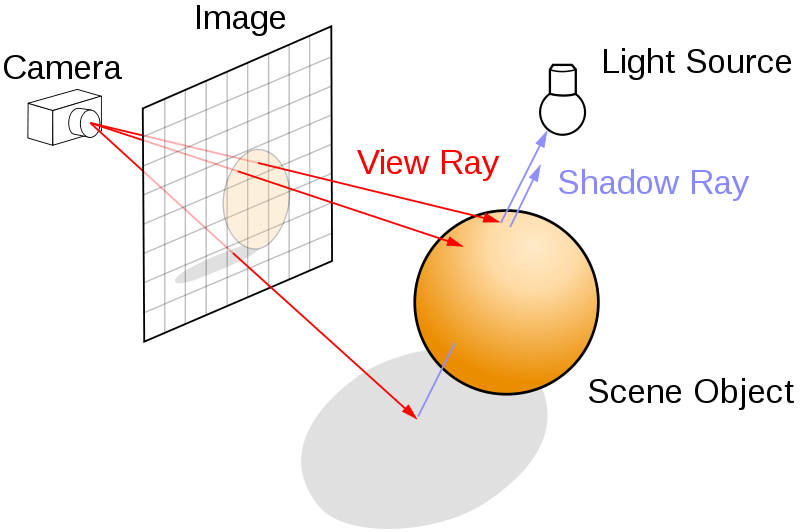
\includegraphics[height=3.0in]{figures/Ray_trace_diagram.png}
\caption{Ray Tracing Diagram\cite{RayTracingDiagram}}
\label{fig:raytracingdiagram}
\end{figure}

\section{Direct Illumination: Ray Casting}
\label{sec:RayCasting}
For this thesis, direct illumination encapsulates the ray casting process. Direct illumination will is referred to as illumination that emanates from a virtual light in a 3D scene that contributes to a 3D object's final color in addition to that object's material attributes.  Direct illumination also encompasses an image's shadowing information, which is an obstruction in the light ray-object intersection.

Ray casting, a term first introduced by Scott Roth in 1982, is the process of casting rays into a 3D scene, finding the closest intersection from the eye/camera through boolean operations, and returning the color value of that object\cite{Roth1982}.  By emulating the different properties of light based on the cosine of the normal vector and the normalized vector from the high point of the object to a light, semi-realistic results are produced.  Other, more cartoon-ish, effects are created using similar methods, most notably Gooch and Gooch shading.

For this research, the basic Phong model of shading was used to generate specular highlights on 3D objects. This model, which has been altered slightly by Jim Blinn, will be discussed fully in following sections.  The Phong model equation is for a ray intersecting the surface of an object at point ~$P$ as follows:

\begin{equation}
\label{eq:phongModel}
color_{output} = k_{d}O_{d}I_{a} + k_{d}O_{d}I_{d}[\hat{L_{m}} \cdot \hat{N}] + k_{s}O_{s}[\hat{R_{m}} \cdot \hat{V}]^{n}I_{d} \cite{hughes2013computer}
\end{equation}

where ~$k_{d}$ and ~$k_{s}$ are the diffuse and specular reflection coefficients, ~$I_{a}$ is the ambient light color, ~$I_{d}$ is the diffuse light color, ~$O_{d}$ is the diffuse color of the object, ~$L_m$ is the direction vector from point ~$P$ towards the light, ~$N$ is the surface normal for the surface at ~$P$, ~$O_{s}$ is the specular color of the object, ~$R_m$ is the direction that a perfectly reflected ray of light would take from ~$P$, and ~$n$ is the specular exponent, or shininess.  Each part of this equation will be discussed.  The second part of the equation,  ~$k_{d}O_{d}I_{d}[\hat{L_{m}} \cdot \hat{N}]$,  can be easily defined with Lambert shading.

\subsection{Lambert Shading}
\label{subsec: Lambert Shading}
\begin{figure}[h]
\centering
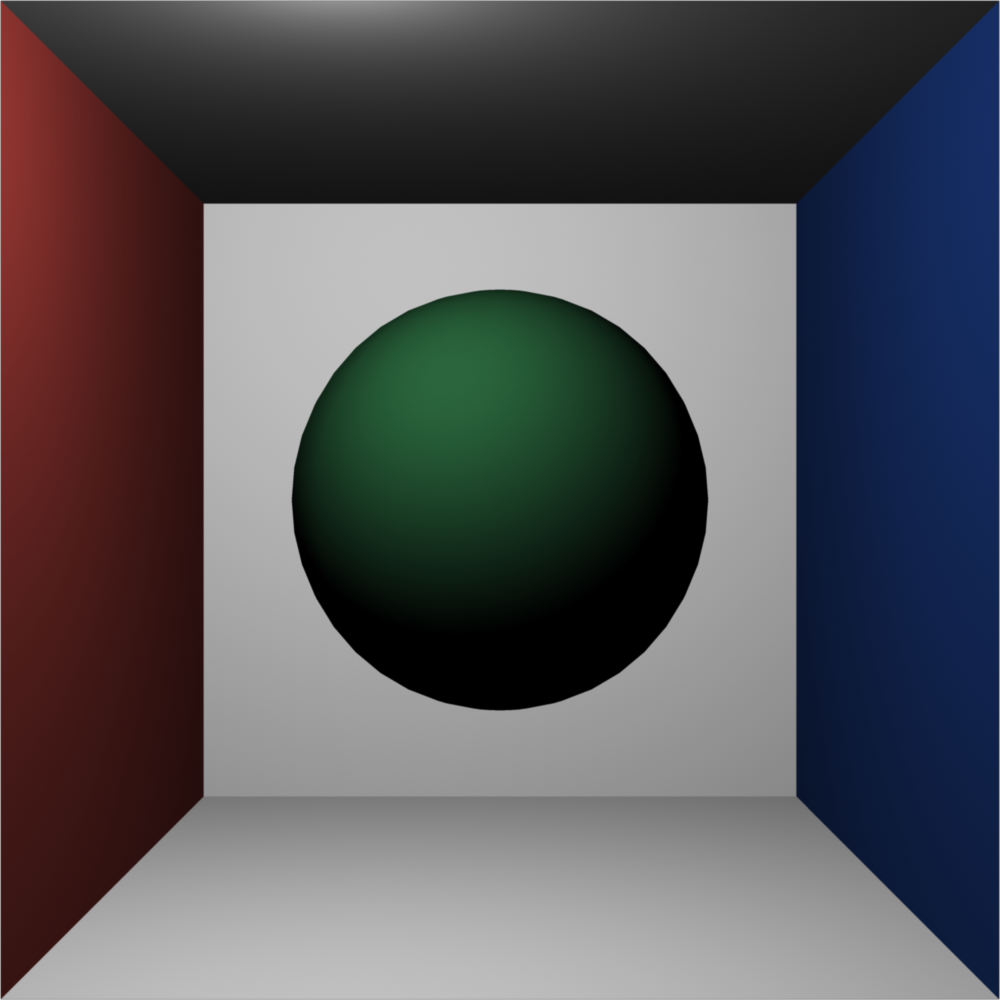
\includegraphics[height=3.0in]{figures/lambert_Maya.png}
\caption{An example of Lambert Shading created in Autodesk Maya 2010\copyright}
\label{fig:lambertmaya}
\end{figure}
The Lambertian model for reflectance is the diffuse component of a surface's material, or the diffuse reflection of a material's properties.  Diffuse objects are generally thought of as anything that does not reflect light off of its surface, such as unfinished wood.  This effect can be see in Figure \ref{fig:lambertmaya}. This model follows Lambert's cosine law for optics, which states that the radian intensity or luminous intensity observed from an ideal diffusely reflecting surface or ideal diffuse radiator is directly proportional to the cosine of the angle ~$\theta$ between the observer's line of sight and the surface normal.  Applying this law to computer graphics we the following equation:

\begin{equation}
\label{eq:lambert}
color_{output} = \hat{L_{m}} \cdot \hat{N} CI_{L}
\end{equation}

where ~$\hat{L_{m}}$ is the normalized direction of the light-direction vector, ~$\hat{N}$ is the normalized normal vector, ~$C$ is the color, and ~$I_{L}$ is the intensity of the incoming light.  Since ~$L \cdot N =  |N||L|\cos{\theta}$, if we make the lengths of ~$|N||L| = 1$ by normalizing them, equation \ref{eq:lambert} satisfies the properties for Lambertian shading by making ~$L \cdot N = \cos(\theta)$.  As we can see, Equation \ref{eq:lambert} is actually the term represented as ~$k_{d}O_{d}I_{d}[\hat{L_{m}} \cdot \hat{N}]$ in Equation \ref{eq:phongModel}, where ~$C = O_{d}$ and ~$I_{L} = I_{d}$.

\subsection{Gouraud Shading}
\label{subsec: Gouraud Shading}
One of the first shading paradigms introduced to the computer graphics community was a vertex interpolation shading created by Henrik Gouraud at the University of Utah\cite{gouraud1971}.  Gouraud's algorithm successfully captured the Lambertian Shading effect described in Section \ref{subsec: Lambert Shading}.  Gouraud's approach saved intensity values at each vertex as a weighted average of the normals of the surrounding polygons in the object's mesh.  When a hit on an object was achieved, a weighted sum of the point's color was returned depending on the intensity values at each closest vertex.  This effect is demonstrated in Figure \ref{fig:gouraudMaya}.
\begin{figure}[h]
\centering
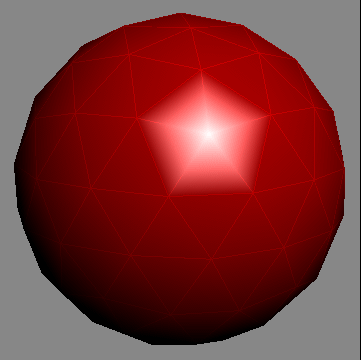
\includegraphics[height=3.0in]{figures/gouraud_low.png}
\caption{An example of the deficit of Gouraud shading being apparent in the highlight in a lowpoly model.\cite{GouraudLow} }
\label{fig:gouraudMaya}
\end{figure}

While this method works well,  it is also dependent on the density of the object's mesh since each vertex intensity is basically an average of the surrounding normals.  This technique also benefits from the relatively simple calculations needed per hit point because, generally speaking, a polygon is made up of a 3 or 4 vertexes maximum.  Instead of calculating Equation \ref{eq:phongModel} at each pixel of intersection within the scene, interpolation between precalculated vertex intensities is needed.  Unfortunately, since the smooth perception of shading is based off of interpolation, which in effect is characterized by the density of object meshes, high localized specular highlights will not be rendered correctly.  Also, if a highlight lies in the middle of a polygon, but does not spread to the polygon's vertex, it will not be apparent in the render.  If the highlight appears directly on a vertex, while it will be rendered correctly for that vertex, it will be rendered incorrectly on neighboring polygons. An example of this deficit for Gouraud's shading can be see in Figure \ref{fig:gouraudMaya}.  For this reason, Equation \ref{eq:phongModel} was introduced.

\subsection{Phong Shading}
\label{subsec:Phong Shading}
\begin{figure}[h]
\centering
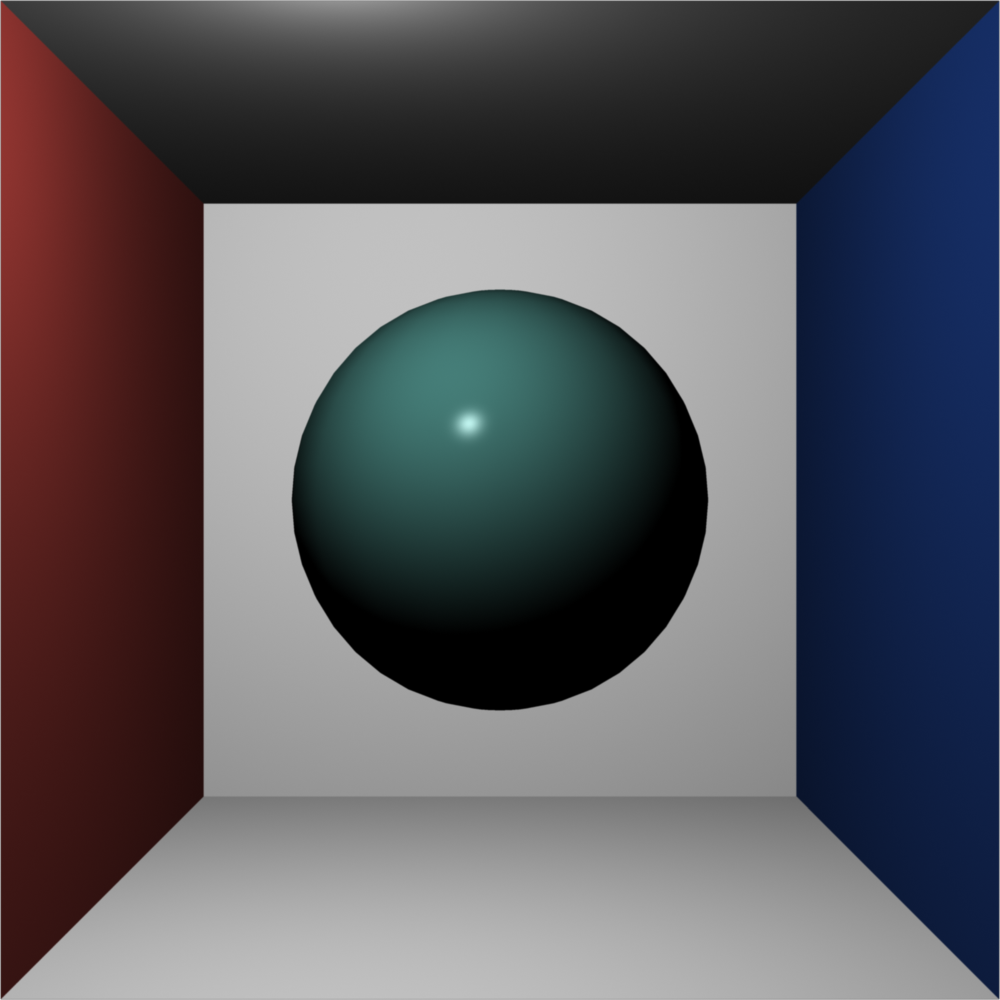
\includegraphics[height=3.0in]{figures/phong_Maya.png}
\caption{Phong Shading created in Autodesk Maya\copyright 2010}
\label{fig:phongmaya}
\end{figure}
Another aspect of an object's illumination model is the specular component of an object.  Specularity is the visual appearance of specular reflections.  This represents an object's ``shininess".  One strategy to display this specular highlight was introduced by Bui Tuong Phong \cite{Phong1975}. Whereas Phong's predecessors interpolated across surface patches \cite{gouraud1971}, as stated in Section \ref{subsec: Gouraud Shading}, Phong interpolated surface normals and evaluated a lighting model at each pixel.  He also added a specular component to the lighting model to produce highlights.\cite{lyon1993phong}

Phong's specular component from his paper \textit{Illumination for Computer-Generated Images} introduces the equation at ray-object intersection point ~$P$:

\begin{equation}
\label{eq:Phong01}
color = C_{p}[\cos{i} + d] + W(i)[\cos{s}]^{n}
\end{equation}

where~$C_p$ is the reflection coefficient of the object at point ~$P$,~$i$ is the incident angle,~$d$ is the environmental diffuse reflection coefficient, ~$W(i)$ is a function which gives the ratio of the specular reflected light and the incident light as a function of the incident angle ~$i$, and ~$s$ is the angle between the direction of the reflected light and the light of sight.

The important aspect of Equation \ref{eq:Phong01} is the term ~$[\cos(s)]^{n}$.  Since the cosine of the angle between the direction of the reflected light, or ~$R_{m}$ in Equation \ref{eq:phongModel}, and the line of sight, ~$V$, is equal to ~$R_{m} \cdot V$ as long as each vector is of unit length, we only need to know what ~$R_{m}$ is.

To calculate ~$R_{m}$ we have this equation from Phong as well\cite{lyon1993phong} at ray-object intersection point ~$P$:
\begin{equation}
\label{eq:phongreflect}
R_m = 2[L_m \cdot N]N - L_m
\end{equation}

where ~$L_{m}$ is the direction vector from ~$P$ towards the light and ~$N$ is the surface normal at ~$P$.  The effect of Phong shading can be seen in Figure \ref{fig:phongmaya}.

\subsection{Blinn Shading}
\label{subsec:Blinn Shading}
\begin{figure}[h]
\centering
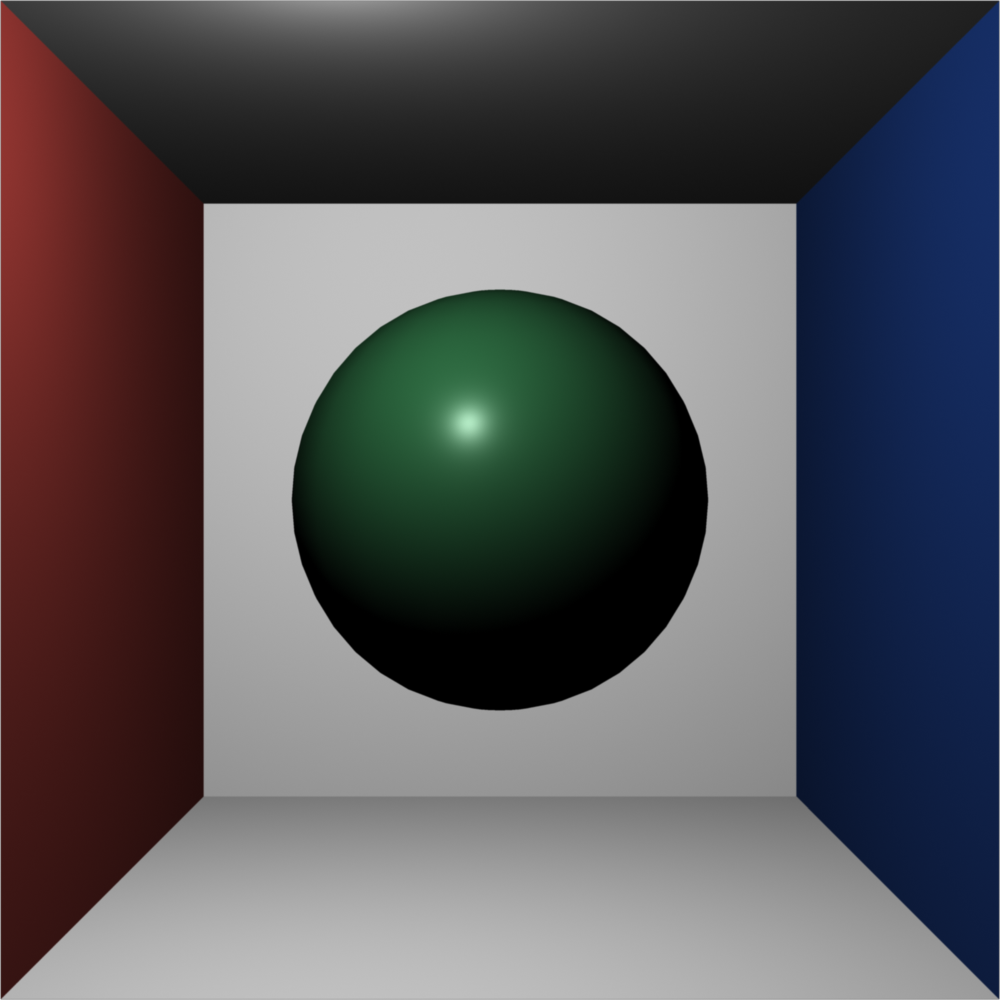
\includegraphics[height=3.0in]{figures/blinn_Maya.png}
\caption{Blinn Shading created in Autodesk Maya 2010\copyright}
\label{fig:gooch}
\end{figure}
In Jim Blinn's paper \textit{Models of Light Reflection for Computer Synthesized Pictures} he introduces the equation\cite{Blinn:1977}:

\begin{equation}
\label{eq:blinnModel01}
color = p_{a} + max(0,N\cdot L) p_{d} +  (N \cdot H)^n p_{s}
\end{equation}
which is most similar to Equation \ref{eq:phongModel} because of its ambient term ~$p_{a}$, diffuse term ~$p_{d}$ and specular term ~$p_{s}$.  Most importantly for Blinn's equation is the inclusion of ~$H$.  Instead of using Phong's ~$R_{m}$ from Equation \ref{eq:phongreflect}, Blinn introduces a new half-vector called ~$H$.  Blinn describes,

\begin{quote}
``If the surface was a perfect mirror, light would only reach the eye if the surface normal, ~$N$, pointed halfway between the source direction, ~$L$, and the eye direction, ~$E$.  We will name this direction of maximum hilights ~$H$..."
\end{quote}
Relating this to the variables in this paper:
\begin{equation}
\label{eq:BlinnH}
H = \frac{\hat{L} + \hat{V}}{len(L+V)}
\end{equation}

Equation \ref{eq:BlinnH} then replaces ~$R \cdot V$ in Equation \ref{eq:phongModel}.  Blinn's model produces more accurate models of empirically determined  bidirectional reflectance distribution functions for many different types of surfaces\cite{ngan2004experimental}.  While this equation produces better results, it also introduces a square root math function when determining  ~$len(L+V)$.  Since a square root calculation takes more time than a dot product calculation, Blinn's model has been considered slower.(With computer processing achievements today, however, the speed differences are incomparable.)  Although it will not be used in this thesis, I hvae included it to help show the origins of Equation \ref{eq:phongModel}.

\subsection{Gooch and Gooch Shading}
\label{subsec:GoochShading}
\begin{figure}[h]
\centering
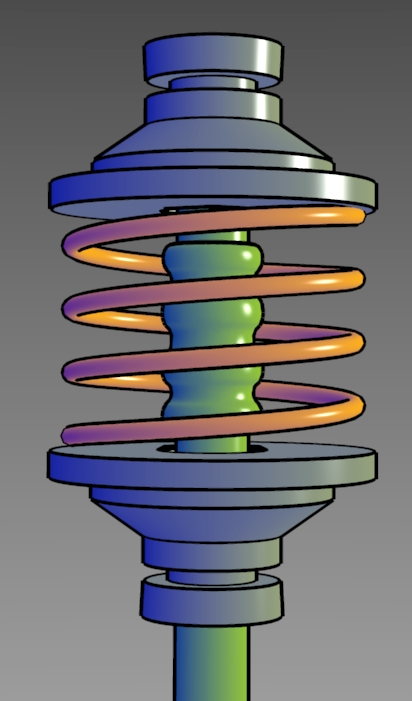
\includegraphics[height=3.0in]{figures/gooch.jpg}
\caption{Gooch Shading Example\cite{gooch1998non}}
\label{fig:gooch}
\end{figure}
Ever since the introduction of Phong's model for photo-realistic rendering of geometric objects, there has been a trend towards non-photorealistic rendering(NPR).  Most notable in this field is the work of Amy and Bruce Gooch, et al.  Gooch and Gooch argue that ``Phong shaded 3D imagery does not provide geometric information of the same richness as human-drawn technical illustration\cite{gooch1998non}."    NPR techniques are referred to as computer graphics algorithms that imitate traditional techniques such as painting or pen-and-ink\cite{gooch1998non}.  Gooch, et al. introduced a generalization of the classic computer graphics equation from Equation \ref{eq:lambert} by experimenting with the value of ~$L_{m} \cdot N$.  Their equation is as follows:

\begin{equation}
\label{eq:Gooch&Gooch}
color = \left(\frac{1 + (\hat{L_{m}} \cdot \hat{N})}{2}\right) k_{cool} + \left(1-\frac{1 + (\hat{L_{m}} \cdot \hat{N})}{2}\right) k_{warm}
\end{equation}
where ~$k_{cool}$ and ~$k_{warm}$ are two color values to interpolate between. In Equation \ref{eq:Gooch&Gooch}, they use the large fractions to remap the values of ~$\hat{L_{m}} \cdot \hat{N}$ between zero and one, causing the colors to gracefully blend from ~$k_{cool}$ to ~$k_{warm}$.  As can be seen in Figure \ref{fig:gooch}, the Gooch shading algorithm also includes outlines around each shape.  Gooch referred to creating the outline in the paper \textit{Real-Time Nonphotorealistic Rendering}\cite{markosian1997real}, but for this thesis the outline is determined from when the values of ~$\hat{L_{m}} \cdot \hat{N}$, after being remapped between 0 and 1, are between a certain threshold and zero.  While this may not the best way to generate outlines around 3D shapes, it accomplishes semi-reliable results and was therefore utilized in this thesis.
\subsection{Texture Mapping and UV Coordinates}
\label{subsec:TexMap}
\begin{figure}[h]
\centering
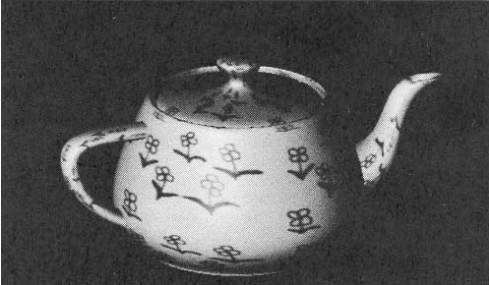
\includegraphics[height=2.0in]{figures/flowerteapot.png}
\caption{An example of texture mapping to the surface of a teapot. \cite{blinn1976texture}}
\label{fig:teapot}
\end{figure}
Up to this point, we've focused on explaining basic color appropriation with solid colors represented as RGB; in computer graphics,however, it is also possible to map photographs to the surface of 3D objects.  This idea was first introduced by Ed Catmull in 1974 when he demonstrated a method of representing 3D curved patches as opposed to conventional polygons.  This method ``maps" photographs to the surfaces of these patches\cite{catmull1974subdivision}. Jim Blinn expanded this to include environmental mapping based off of reflections from the surface of objects\cite{blinn1976texture}, as can be seen in Figure \ref{fig:teapot}.

\subsubsection{Bump/Normal Mapping}
\label{subsubsec:BNMap}
\begin{figure}[h]
\centering
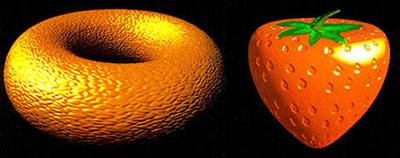
\includegraphics[height=2.0in]{figures/blinn_bump.jpg}
\caption{An example of bump mapping introduced by Jim Blinn. \cite{blinn1978simulation}}
\label{fig:bumpmap}
\end{figure}
As another expansion of Catmull's texture mapping, Blinn also introduced a technique that could simulate a rough or textured surface on a 3D shape, called bump mapping\cite{blinn1976texture}. Blinn discovered that by altering the normal at each point of intersection on the surface of a 3D shape, simulations of wrinkled surfaces can be generated as seen in Figure \ref{fig:bumpmap}.  The normal at each point can be mapped to an image texture or altered via a noise generating equation such as Perlin noise.  Blinn's wrinkled surface simulation can be seen in Figure \ref{fig:bumpmap}.
\section{Ray Tracing and Distributed Ray Tracing}
To improve upon the Phong specular shading model, a new recursive technique was introduced by Turner Whitted at Bell Laboratories.  Turner hypothesized that a tree model should be used to calculate accurate, realistic representations of the physical world's reflective process.  He based his algorithm on an reflection ray, ~$R$, that represents the reflection of a ray on a perfectly smooth surface, and ~$P$, which represents the transmitted ray through a perfectly smooth surface:

\begin{equation}
\label{eq:raytracing1}
\hat{V}' = \frac{\hat{V}}{\hat{V} \cdot \hat{N}}
\end{equation}
\begin{equation}
\label{eq:raytracing2}
\hat{R} = \hat{V}' + 2\hat{N}
\end{equation}
\begin{equation}
\label{eq:raytracing3}
\hat{P} = k_{f}(\hat{N} + \hat{V}') - \hat{N}
\end{equation}
where
\begin{equation}
\label{eq:raytracing4}
k_{f} = (k_{n}^{2}|\hat{V}'|^{2} - |\hat{V}' + \hat{N}'|^2)^{\frac{1}{2}}
\end{equation}

and $k_{n}$ is the index of refraction for the surface.  The equations assume that ${\hat{V} \cdot \hat{N}}$ is less than zero so the sign of ${N}$ must also be adjusted to point to the side of the surface the intersecting angle is incident from. When tracing a ray from the eye point, the intersection at each reflective surface determines the next surface hit, forming a recursive tree formation.  Upon achieving this tree, the following equation calculates the surface color:

\begin{equation}
\label{eq:raytracing5}
color_{output} = I_{a} + k_{d} \sum{j=1}^{j=ls}(\hat{N} \cdot \hat{L_{j}}) + k_{s}S + k_{t}T
\end{equation}
where \newline
\noindent
$S$ = the intensity of light incident from the $\hat{R}$ direction\newline
$k_{t}$ = the transmission coefficient\newline
$T$ = the intensity of light from the $\hat{P}$ direction\newline

By keeping $k_{s}$ and $k_{t}$ constant Turner achieved his results, but for ideal cirumstances the values should be mapped to a Fresnel algorithm that relates them to realistic models of reflection and refraction.

To enhance the raytracing process, Cook, Loren and Carpenter introduced the term ``distributed ray tracing", described as:

\begin{quote}
``...The key is that no extra rays are needed beyond those used for oversampling in space.  For example, rather than taking multiple time samples at every spacial location, the rays are distributed in time so that rays at different spatial locations are traced at different instants of time.
\begin{itemize}
\item Sampling the reflected ray according to the specular distribution function produces gloss (blurred reflection)
\item Sampling the transmitted ray produces translucency (blurred transparency).
\item Sampling the solid angle of the light sources produces penumbras.
\item Sampling the camera lens area produces depth of field.
\item Sampling in time produces motion blur."
\end{itemize}
\end{quote}

The introduction of randomization, or jittering, achieves the distributed ray tracing effect. By jittering the ${R}$ value of $T$ in Equation \ref{eq:raytracing5} a glossy effect is produced. The same can be said of the $P$ value from the $T$ variable in Equation \ref{eq:raytracing5}.  Distributed ray tracing is important to a 3D image's realism because it is not possible to achieve the computed perfect reflection/refraction model introduced by Whitted in the natural world.

\section{Indirect Illumination/ Radiosity Effects}
For this thesis, Indirect illumination accounts for any shading or color values not calculated directly from the virtual light in a scene.   These terms are known as ambient occlusion, global illumination and caustic effects. In the natural world, diffuse reflection is the reflection of light from a surface such that an incident ray is reflected at many angles rather than at just one angle, which is the case of specular reflection.  Typically an object will base its final color off of not only the light shining at it, but also from the colors of the objects in closest proximity to it.  This effect is seen in Figure \ref{fig:diffusereflectionrw} in the picture of a racquetball.  The surface of both the racquetball and the piece of paper are as close to Lambertian surfaces as can be found in the natural world.  In the figure the diffuse reflection is most prominent in the racquetball's shadow.  It may seem like a trick on the eyes, but the shadow has a purple tint to it because of the diffusely reflected light rays coming from the racquetball.  In theory, if an object is illuminated in a room with bright red walls the color of the object will have a red tint because of the diffuse reflection of the red from the walls contributing to the overall color of its surface.  It is near impossible to determine all the different contributors to an objects final color in the natural world because of the infinite amount of light rays absorbed and reflected by an object's surface.

\begin{figure}[h]
\centering
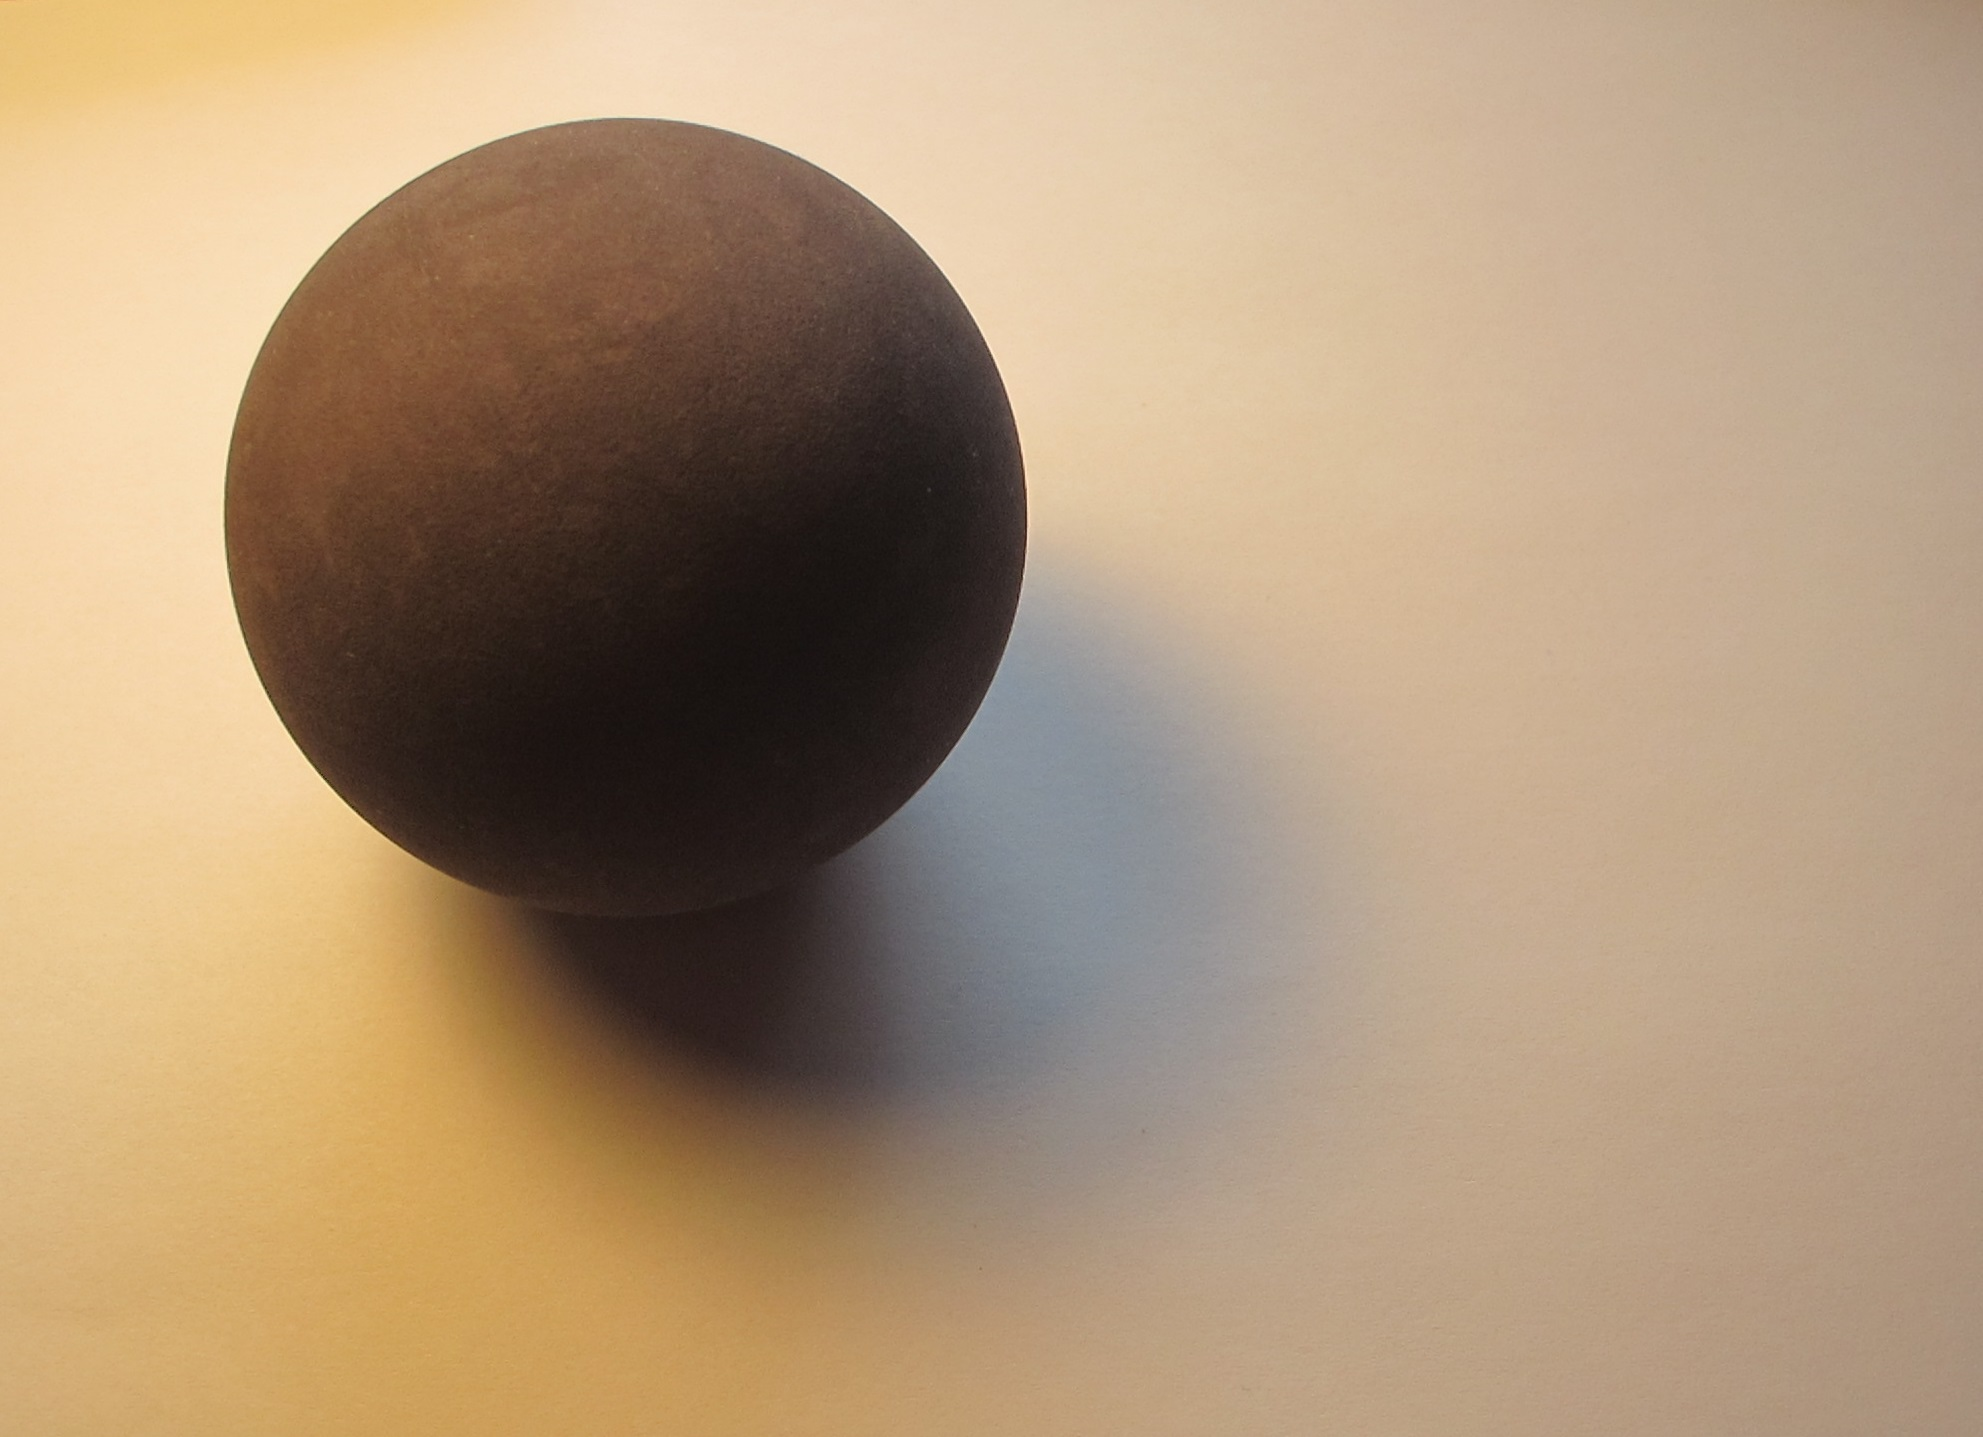
\includegraphics[height=3.0in]{figures/raquetball.JPG}
\caption{Real World Indirect Illumination/Radiosity Effect with a racquetball on a piece of paper.}
\label{fig:diffusereflectionrw}
\end{figure}

To simulate this effect in a 3D environment, new terms were introduced by Torrance, Greenberg et.al \cite{Goral:1984}, who determined a model of light interaction between diffuse surfaces based off of methods used in thermal engineering.  To simplify their method, this thesis used a method inspired by their work.  The process to calculate ambient occulsion, global illumination, and caustic effects are fundamentally all the same.  At each point in a scene, a specific number of sample rays will be cast at each intersection point.  The average of the resulting color information from each sampling ray set determines that pixel's final color.  Ambient occlusion is the simplest.  Ambient occlusion informs the proximity of objects with other objects.  Ambient Occlusions produces a black and white image that will be darker in pixels where images are closer together and lighter in places where images are farther apart.  To calculate this set, one simply needs to determine if another object is hit by a ray in the set or not.  For instance, if 255 rays are cast from an object, and 200 of them hit another object in a distance greater than 0, then the value for that pixel will be 200/255 or .7843.  An ambient occlusion example can be seen in Figure \ref{fig:aOcclusion}.

\begin{figure}[h]
\centering
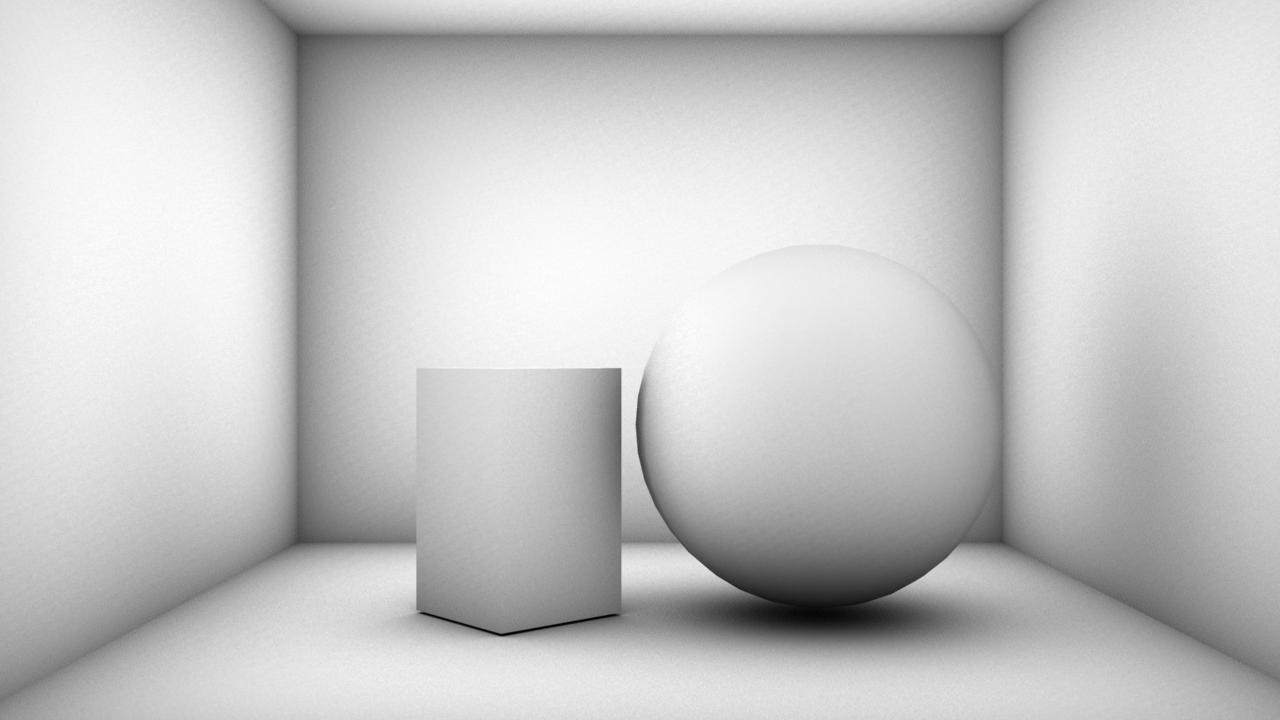
\includegraphics[height=3.0in]{figures/aOcclusion.jpg}
\caption{Example of Ambient Occlusion}
\label{fig:aOcclusion}
\end{figure}

To calculate global illumination, at each point in the sample set of data, instead of calculating the distance from the point, the direct illumination shading value is added.  Rather than the average number of intersections, the average color is determined from 255 sample rays for a global illumination calculation.  This is seen in Figure \ref{fig:globalill}.  This process is where the color bleeding from nearby objects can best be seen.

\begin{figure}[h]
\centering
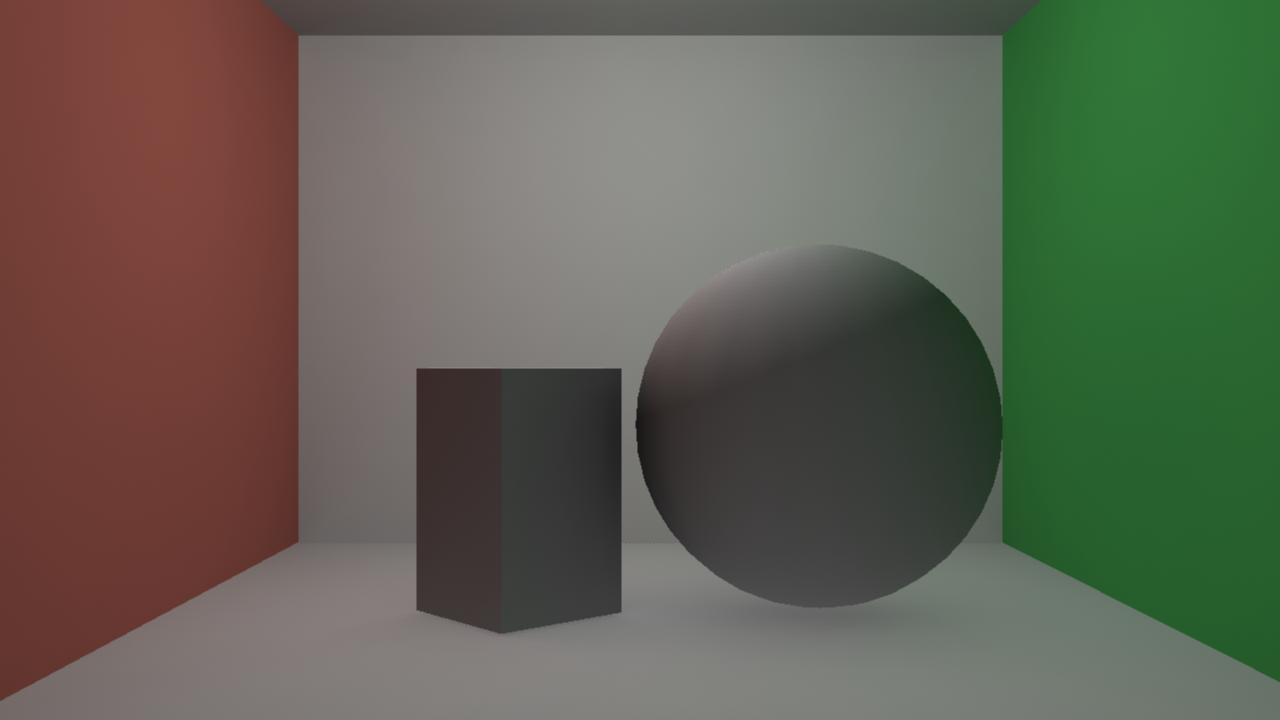
\includegraphics[height=3.0in]{figures/globalIll.jpg}
\caption{Example of Global Illumination}
\label{fig:globalill}
\end{figure}

The final effect is a caustic, which is the ratio of specular color at each point on a surface.  If a surface receives caustics, it calculates the reflective rays of nearby objects and returns the reflected color value average for each sample ray set.  This effect is seen in Figure \ref{fig:caustics}.
\begin{figure}[h]
\centering
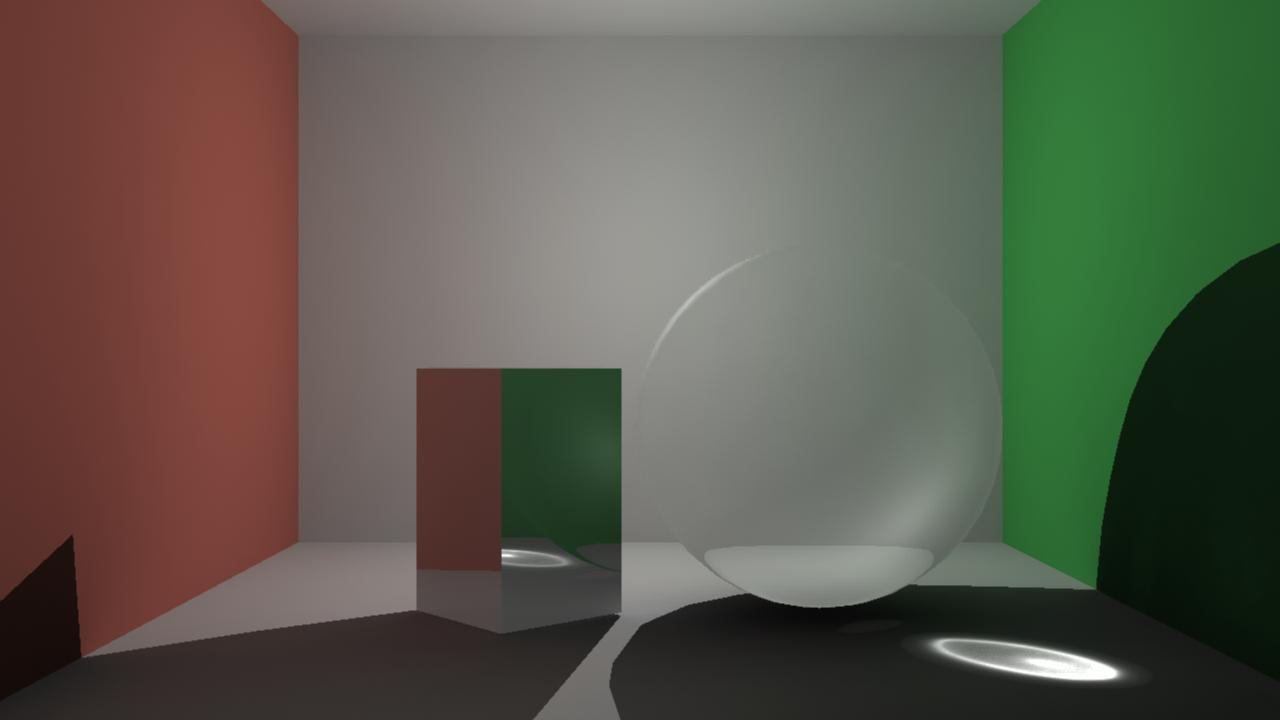
\includegraphics[height=3.0in]{figures/caustics.jpg}
\caption{Example of Caustic Effect}
\label{fig:caustics}
\end{figure}

Indirect illumination combined with distributed ray tracing has made a difference in the realistic perception of generated photorealistic images, and an effort is being made to incorporate these effects into realtime settings like video games in order to provide a more immersive experience.  Large sample ray sets are needed for more realistic looking images however, and the computing power required to produce this effect in realtime is sizable and expensive.

\section{Languages}
The four languages I evaluated were determined for specific reasons.  They had to have the ability to follow the object-oriented paradigm and possess the potential to perform graphical methods like imaged reading and writing.  A brief history behind each language will be discussed to give insight into the basis for each language's creation, which will also provide insight as to their feasibility in creating an image synthesis program.
\subsection{C++}
\label{sub:C++}
C++ is a general-purpose object-oriented coding language.  Its genesis lies in research done with the programming \textit{C with Classes} in 1979, although its commercial release was not until October 1985\cite{stroustrup1996history}. C++ is considered an intermediate-level language because of its capabilities with both high and low level computer functionality.  Creator Bjarne Stroustrup claims to have drawn inspiration from not only C, but also from Simula, Algol68, BCPL, Ada, CLU and ML.  Since its creation, C++ has gone on to influence the creation of numerous coding languages, such as C\#\cite{naugler2007c}.

According to Stroustrup, C++ was originally designed to combine Simula's facilities for program organization with C's efficiency and flexibility for systems programming\cite{stroustrup1996history}.  C++ is an extension of the C programming language. In fact, it stemmed from a fundamental design called \textit{C with Classes}\cite{stroustrup1996history}.  When Stroustrup designed the C++ language he had a variety of guidelines he deemed as ``suitable" for computer languages.  He writes:
\begin{quote}
\label{qt: StroustrupC++History}
\begin{enumerate}[label = {[\arabic*]}]
\item `` A good tool would have Simula's support for program organization- that is, classes, some form of class hierarchies, some form of support for concurrency, and strong(that is, static) checking of a type system based on classes.  This I saw as support for the process of inventing programs, as support for design rather than just support for implementation.

 \item A good tool would produce programs that ran as fast as BCPL programs and share BCPL's ability to easily combine separately compiled units into a program.  A simple linkage convention is essential for combining units written in languages such as C, Algol168, Fortran, BCPL, assembler, etc., into a single program and thus not get caught by inherent limitation in a single language

 \item A good tool should also allow for highly portable implementations.  My experience was the ``good" implementation I needed would typically not be available until ``next" year and only on a machine I couldn't afford....\cite{stroustrup1996history}"
\end{enumerate}
\end{quote}
To further emphasize C++'s benefits, Stroustrup explained why he chose C over other languages of the time to build upon:
\begin{quote}
\label{q:StroustrupCvsOther}
``C is clearly not the cleanest language ever designed nor the easiest to use so why do so many people use it?
\begin{enumerate}[label = {[\arabic*]}]
\item C is \textit{flexible}: It is possible to apply C to most every application area, and to use most every programming technique with C.  The language has no inherent limitations that preclude particular kinds of programs from being written.
\item C is \textit{efficient}:The semantics of C are ``low level"; that is, the fundamental concepts of C mirror the fundamental concepts of a traditional computer.  Consequently, it is relatively easy for a compiler and/or a programmer to efficiently utilize hardware resources for a C program.
\item C is \textit{available}: Given a computer, whether the tiniest micro or the largest super-computer, the chance is that there is an acceptable quality C compiler available and that that C compiler supports an acceptably complete and standard C language and library.  There are also library and support tools available, so that a programmer rarely needs to design a new system from scratch.
\item C is \textit{portable}: A C program is not automatically portable from one machine (and operating system) to another nor is such a port necessarily easy to do.  It is, however, usually possible and the level of difficulty is such that porting even major pieces of software with inherent machine dependencies is typically technically and economically feasible.
\end{enumerate}
Compared with these ``first order" advantages, the ``second order" drawbacks like the curious C declarator syntax and the lack of safety of some language constructs become less important. Designing ``a better C" implies compensating for the major problems involved in writing, debugging, and maintaining C programs without compromising the advantages of C. C++ preserves all these advantages and compatibility with C at the cost of abandoning claims to perfection and of some compiler and language complexity. However, designing a language ``from scratch" does not ensure perfection, and the C++ compilers compare favorably in run−time, have better error detection and reporting, and equal the C compilers in code quality. \cite{stroustrup1996history}"
\end{quote}
Stroustrup sought to create a universal, object-oriented language that was accessible and relatively low maintenance to begin programming with since most computers were, and still are, compatible with C.

Object-oriented programming provides clean and modular code that is easier to maintain and debug, because it separates functions and utilities into class objects, which can be reused.  This is C++'s main benefit to the image synthesis process, in addition to its efficiency in utilizing hardware resources from a computer to provide faster results.

\subsection{Processing}
\label{sub:Processing}
Processing is an open-source programming language and integrated development environment, or IDE, developed by Casey Reas and Benjamin Fry in 2001. According to the Processing website (processing.org):
\begin{quote}
``Processing is a programming language, development environment, and online community.  Since 2001, Processing has promoted software literacy within the visual arts and visual literacy within technology.  Initially created to serve as a software sketchbook and to teach computer programming within a visual context, Processing evolved into a development tool for professionals.  Today there are tens of thousands of students, artists, designers, researchers and hobbyists who use Processing for learning, prototyping and production."
\end{quote}

Andrew Glassner, a pioneer in Ray Tracing, also wrote a book on Processing called \textit{Processing for Visual Artists}.  Glassner helps to emphasize the importance and use for Processing in the visual world:

\begin{quote}
``Processing is for artists, designers, visualization creators, hobbyists or anyone else looking to create images, animation, and interactive pieces for art, education, science or business....Processing offers you a 21st-century medium for expressing new kinds of ideas and engaging audiences in new ways..."
\end{quote}

The usefulness and applicability of Processing in the ray tracing process can be found in its mission statement. It was initially designed to teach computer programming within a visual context.  Since that is also the aim and goal of this thesis, Processing was a reasonable option to investigate. Processing uses Java syntax and packages the java compilation process into its IDE, so a functional overview of Java is also needed to fully determine the usefullness of Processing.

\subsubsection{Java}
%TODO Object-oriented - high Level - cross platform

\subsection{Python}
\label{sub:Python}
Python, named after \textit{Monty Python's Flying Circus}, was first founded by Guido van Rossum.  He began his work on Python at the the National Research Institute for Mathematics and Computer Science in the Netherlands in 1989.  Python is a high-level and interpreted programming language.  While it can be argued that all computer languages are interpreted, Python is considered an interpreted language because unlike C or C++, Python does not require a compiler to operate.  While C and C++ compiled code needs to be compiled into machine-language before it is relayed to the computer, Python's instructions are interpreted directly from its written code.  van Rossum is quoted as saying he was unhappy with the productivity of creating a script or utility in C, which influenced his interest in establishing Python\cite{vanBlog1}.

One of the main focuses of Python is readable syntax.  According to Jim Mcconnell's book \textit{Code Complete}, one line of Python is equivalent to six lines of C code\cite{mcconnell2004code}.  According to van Rossum, Python's creation was heavily influenced by the coding language ABC.  ABC's design was intended to be a programming language that could be taught to intelligent computer users who were not computer programmers or software developers.  The main deficit with ABC's design was its inability to bridge the gap in GUI creation and an inability to directly access the file system and operating system in a computer.  Python's syntax eliminates the need for traditional curly braces (\{\}) and instead uses a tabular system that denotes code blocks.
\subsection{RenderMan}
\label{sub:RenderMan}
RenderMan\copyright\space is a software and application programming interface, or API, that many companies in the computer industry use to render large projects for entertainment or video game use.  RenderMan\copyright\space specializes in network distribution of renderings throughout a ``renderfarm" that has the ability to render ray traced images faster than a single computer.  RenderMan\copyright\space is referred to as the rendering engine that produces the image.  RenderMan\copyright\space is dependent on two files: RenderMan\copyright\space Interface Bytestream (RIB) and RenderMan\copyright\space shading file.  RIB acts as a descriptor for how the engine should work, incorporating all aspects of ray casting, ray tracing, direct illumination, distributed ray casting, and direct illumination.  A shading file is written in the RenderMan\copyright\space Shading Language (RSL), and acts as a description file for how objects in a scene interact with light.  By utilizing the RIB and RSL files, each ray tracing milestone was accomplished within the scope of this thesis.

It is important to note that RenderMan\copyright\space has already implemented all of the milestones needed for this thesis.  Also, RenderMan\copyright\space is based off of a camera projection matrix algorithm that does not cast rays the same way that this thesis does ray casting.  RenderMan\copyright\space also incorporates a variety of highly advanced rendering techniques that are too far outside the scope of this modest master's thesis to discuss.  The thesis will discuss the feasibility of utilizing the pre-constructed implementations of the milestones without the aid of production software such as Autodesk Maya\copyright\space or  Side Effects Houdini\copyright\space. This will present the same types of implementation issues that C++, Processing, and Python would in regards to the theory of ray casting. 
%%%%%%%%%%%%%%%%%%%%%%%%%%%%%%%%%%%%%%%%%%%%%%%%%%%
%
%  New template code for TAMU Theses and Dissertations starting Fall 2012.
%  For more info about this template or the
%  TAMU LaTeX User's Group, see http://www.howdy.me/.
%
%  Author: Wendy Lynn Turner
%	 Version 1.0
%  Last updated 8/5/2012
%
%%%%%%%%%%%%%%%%%%%%%%%%%%%%%%%%%%%%%%%%%%%%%%%%%%%

%%%%%%%%%%%%%%%%%%%%%%%%%%%%%%%%%%%%%%%%%%%%%%%%%%%%%%%%%%%%%%%%%%%%%%%
%%%                           METHODOLOGY
%%%%%%%%%%%%%%%%%%%%%%%%%%%%%%%%%%%%%%%%%%%%%%%%%%%%%%%%%%%%%%%%%%%%%%

\chapter{\uppercase {Methodology}}
The methods I used were straightforward.  For each programming language notes were kept that outlined the difficulties and roadblocks caused specific to the language.  The same programming theories and fundamentals were utilized in order to provide continuity between each programming process.  Due to its helpfulness in managing and organizing large coding projects, the object-oriented approach to programming was taken.  This means that classes with specific variables and data-structures were defined so that instances of objects could be constructed at runtime.  Wherever possible, the image synthesis process was sub-categorized in order to better organize the information needed for the process. This led to shorter development time and also contributed to quicker troubleshooting after the code was written.

The program written for each language used a similar data structure and was modelled after the same overall design.  For each language a similar data structure was also strived for, shown in Figure \ref{fig:RayTracerDataStructure}.

A dynamic data structure that resizes as objects are added or removed along with an agnostic data type was desired for this project.  As we discussed next section, this approach provided a solution that mirrored the functionality of a ray caster.

In addition to having a program architecture and data structure, the milestones I established that segment image synthesis theory within four categories also provided a structured approach to analyzing and reporting the conclusions used for each language. Since each program was modeled after this conceptualization, measurements of success and difficulty were more clearly defined. More details on the milestones are discussed in the following section.

By determining the level of difficulty of implementing the program's data structures and class design, not to mention using that design to further implement the image synthesis milestones of Preliminary Preparations, Direct Illumination, Ray Tracing/Distributed Ray Tracing, and Indirect Illumination, a detailed report has been compiled that informs the results collected and reported in this thesis, all found in the next section.
%%%%%%%%%%%%%%%%%%%%%%%%%%%%%%%%%%%%%%%%%%%%%%%%%%%
%
%  New template code for TAMU Theses and Dissertations starting Fall 2012.
%  For more info about this template or the
%  TAMU LaTeX User's Group, see http://www.howdy.me/.
%
%  Author: Wendy Lynn Turner
%	 Version 1.0
%  Last updated 8/5/2012
%
%%%%%%%%%%%%%%%%%%%%%%%%%%%%%%%%%%%%%%%%%%%%%%%%%%%

%%%%%%%%%%%%%%%%%%%%%%%%%%%%%%%%%%%%%%%%%%%%%%%%%%%%%%%%%%%%%%%%%%%%%%%
%%%                           Implementation
%%%%%%%%%%%%%%%%%%%%%%%%%%%%%%%%%%%%%%%%%%%%%%%%%%%%%%%%%%%%%%%%%%%%%%

\chapter{\uppercase {Implementation Results}}

\section{Image Synthesis Program Structure and Implementation}

The basis for every ray tracing program can be broken down into a simple set of processes.  First, a program must be able to read and write images.  Once the ability to read and write images has been realized, the process for casting rays can begin. This process is demonstrated by the following pseudocode, or code outline:

\begin{algorithm}[H]
\label{alg:RayTracingPseudocode}
\setstretch{1.0}
 \ForEach{~$pixel$ in ~$image$}{
    \ForEach{$object$ in $scene$}{
        \If{$object$ intersects $ray$}{
               $intersectionDistance$ = distance of viewpoint from intersection of object and ray\;
            \If{$intersection$ \space\textgreater\space $previousIntersection$}{
                $previousIntersection$ = $intersection$\;
                }
                }
    }
    \If{$intersection$ exists}{
        \ForEach{~$Light$ in ~$scene$}{
            determine $materialColor$ from ~$light$\;
        }
        $pixel$ = $materialColor$\;
    }
    \Else{
        $pixel$ = black or alpha(no color)
    }
}
write image\;
\caption{Ray Casting Pseudocode}
\end{algorithm}

Each pixel in an image will correspond to a position in 3D space, as demonstrated in Figure \ref{fig:raytracingdiagram}, found on page \pageref{fig:raytracingdiagram}. In this figure, each box represents an image pixel.  To determine each pixel's final color, one must first determine if there is an intersection with any of the 3D objects in a scene and if so, which object is closest.  Then, that object's illumination algorithm must be run, factoring in the light source(s) in the scene.  Each ray tracer written followed these steps, as detailed in Algorithm \ref{alg:RayTracingPseudocode}, but each ray tracer also adheres to specific structure and code organization.  In order to better understand the ray tracing structure, I needed to establish and learn some important Computer Science terms as part of the preliminary preparations for the project.

\section{Milestone 1: Preliminary Preparations}
\label{Milestone1}
\begin{figure}[ht]
\centering
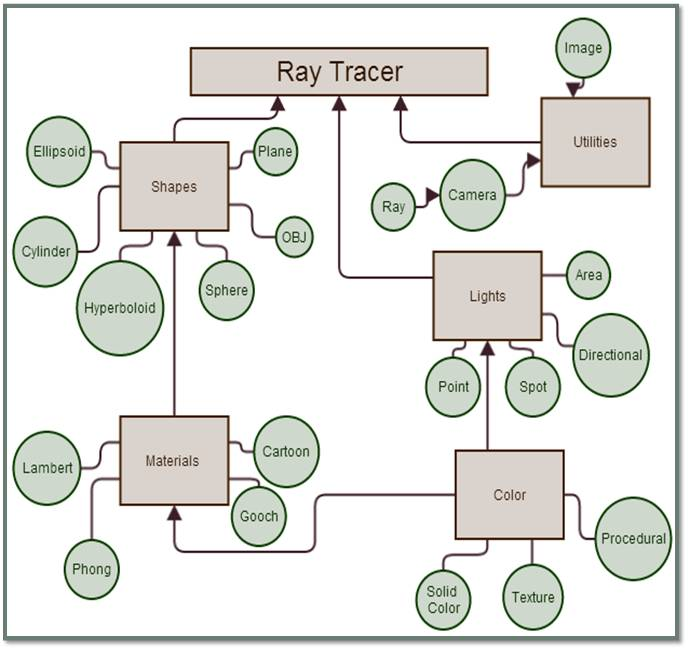
\includegraphics[height=3.0in]{figures/rayTracerStructure.jpg}
\caption{Diagram of the Parenting/Dependency Structure of the Ray Casting Program}
\label{fig:RayTracerDependencies}
\end{figure}
Preliminary preparations refers to anything that needed to be accomplished before being able to start coding the ray tracing theory coding.  In this section, simple matters such as program language installation and accessibility will be discussed.  Also discussed is the majority of the ``Utilities" section of Figure \ref{fig:RayTracerDependencies}.

The foundations of a ray tracing program are built around two fundamental procedures: image writing and vector math. Ray tracing can also be accomplished through matrix operations, but for the purposes of this thesis, vector math will be sufficient.  Vector math is the basis for all ray tracing theory. As such, a class or data structure that can accomplish all aspects of vector math including addition, subtraction, dot product, and cross product is crucial to accomplishing the image synthesis program.  In addition to this, in order to see the final product after all the calculations have been run, you must be able to write an image.  Arguably the easiest image file to write out is a Portable PixMap (PPM).  Other image formats include JPEG, BITMAP, and PNG.  Each of these image formats requires a more complicated compression algorithm than PPM.  Each programming language may also require additional files in order to compile or execute the final product.  Each of these languages will be assessed from the viewpoint of a student in the Visualization Department of Texas A\&M, because this is directly relevant to the my experience.
\subsection{C++}
The C++ language, as described in Section \ref{sub:C++}, is an object-oriented language that is considered both a high and low level language because of the level of control it provides over computer functionalities.  Development and installation with C++ was accomplished via the provided computers at Texas A\&M's Department of Visualization.

When developing in a Linux/Unix environment, C++ can be executed directly from the terminal of the operating system.  This means no external IDE is needed to compile your code.  This development environment was more appealing to me because IDE environments have their own learning curve, which would have to be realized in addition to learning the C++ language semantics.  If a Department of Visualization computer was not available, installation of the C++ development tools would present its own challenges.

To work on a Windows computer, you must first determine which compiler to work from, download that compiler, and then work from that specific compiler's commandline.  Common practice would be to download an IDE such as Visual Studio or Eclipse.  Since computers are not typically sold with a Linux operating system installed on them, developing in Linux outside of an academic setting would require installing a new operating system, which is not a task for beginners.  After learning how to install Linux, you must then learn the proper way to download specific compiler packages. Since this can be accomplished by simply typing a command into the computer's terminal, it can be significantly easier to learn how to do than installing a compiler on Windows.  A Macintosh computer was not tested, but since their operating systems are a variation of the Unix platform much like Linux, and since they are more commonly sold in stores, they are more accessible to students who are not computer scientists.  Starting to develop in C++ on any computer is a complicated task unless a ready-made environment has been provided for you, like at Texas A\&M.

What makes C++ unique from other languages explored in this thesis is the concept of a makefile, and the make command. In order to communicate with the compiler installed on the Unix platform, you need to create a file that will define which source code files are needed to make object files and which compilers and linkers are included in the make command.  A properly configured IDE it will automatically generate a makefile and perform the make command for you.  This further solidified my decision to work without a IDE and use a syntax highlighting text-editor, because nothing was generated automatically. That way, only what was typed and developed by myself was included in the project.  This allowed for easier debugging of the makefile and make command rather than debugging the IDE's internal processes.

The use of header files is another difference between C++ and the other languages used in this thesis..  When creating a class in C++, it is common practice to outline the class structure in one of these ``header" files. The header file serves as the skeleton of the class structure, while the meat of the class's implementation is fleshed out in a ``.cpp" file.  This is a technique inherited from C coding which was used for older computers that could not support large quantities of memory at the same time.  Computers have improved since and this antiquated practice now further segregates the interface of a class from the implementation of the class rather than save memory space during execution time.  For this thesis only header files were used since speed optimization was not a priority.

In addition to a makefile, another obstacle introduced by C++ was the vector math library.  C++ does not have a standard vector library: the operation needs to be hand-coded in order to be available for use.  A developer has to either implement their own vector math library or borrow a pre-existing library.  This requires additional research or work to write the necessary code.  If a developer is going to borrow code from the Internet, an assessment needs to be made regarding the original writer's accuracy.  Subsequently, knowledge must be gained on how to use the classes and structures defined in the borrowed library.  The vector class used for this thesis was a library circulating amongst the Texas A\&M students that was written by a former faculty member at A\&M: the know source is reputable and the code is trusted to be uselful and correct.

The same obstacle applies to the image reading and writing functionality of an image synthesis program.  There is no standard C++ image library.  Once again, in order to read and write images, a developer needs to either write their own code or borrow an existing third-party library.  For this thesis, a class was written to process .ppm images.  I decided that the effort required to create a custom class to process .ppm images would be less than the effort required to untangle the semantics of linking in a third-party image library.  The .ppm format was chosen because it was the most accessible and simplest format to implement.  The created images needed to be converted to .png or .jpg for use on the web and this was very limiting to the functionality of the final image synthesis program.  The thought of including a third-party library, more specifically the semantics of linking the files correctly in the coding process, seemed more difficult than writing an original class.
\subsection{Processing}
The programming language, Processing, approaches the preliminary preparation milestone in a manner that is significantly different from that of C++.  Whereas I was able to avoid IDE's for C++, doing so with Processing would have proven impossible as it happens to \textit{be} an modified and specially engineered IDE for the Java programming language itself.

Installation of the Processing language is simple.  A compressed application file is downloaded from the processing.org website. Once uncompressed an application file can be clicked and opened.  This starts the Processing application and development can begin.  The processing.org website provides downloads for the three major operating systems, Windows(32-bit and 64-bit), Linux(32-bit and 64-bit) and Mac OS X.  Processing does not require installation so it can be run from anywhere on your computer, which means that Processing can even be saved to, and run from, an external hard drive, allowing the developer to work from any computer without having to reinstall an IDE or compiler. The portability of Processing is convenient for students who may not have a laptop and are forced to switch between workstations.

Processing has a vector math library built into its IDE called PVector.  PVector has extensive documentation on the processing.org website.  Despite this, the syntax of PVector operations is anything but straightforward.  This can best be described with an example.  Consider the C++ equation for determining the hit point along a ray from the ray's origin:
\begin{equation}
\label{eq:C++Equation}
p_{hit} = ray.Origin + t*ray.Direction
\end{equation}

This same equation in PVector would be written:
\begin{equation}
\label{eq:PVectorEquation}
p_{hit} = PVector.add(cast.Origin, PVector.mult(cast.Direction,t))
\end{equation}

Rather than overload the math components of the Vector object, each operator is expressed as a function.  Thus, ``+" becomes ``add" and ``*" becomes ``mult.".  This leads Processing operations to grow long and segmented, which causes confusion for the programmer.  As can be seen in the above example, the C++ syntax in Equation \ref{eq:C++Equation} is much easier to read, understand, and therefore debug, than the Processing syntax in Equation \ref{eq:PVectorEquation}.

In addition to the PVector library, Processing also has included its own image library.  Unlike PVector this image library is very convenient, although no math operations were needed to be performed on image objects.  The PImage library has the ability to save or open any type of common image file, as long as the file type is specified within the command.

Processing introduced another challenge when dealing with color.  Color in Processing is defined as a data type, which is saved as 32-bits of data formatted as AAAAAAAARRRRRRRRGGGGGGGGBBBBBBBB, where (A)lpha, (R)ed, (G)reen, and (B)lue components are all stored as 8 bits of data. Within a ray tracer it is necessary to have access to each individual color value in order to take color averages, since you need to calculate each color value individually.  To extract each color value from the color type a process called bit shifting must occur. This can be shown as follows(example taken from processing.org):

\singlespacing
\begin{lstlisting}[language=Java, caption=Java bit shifting to extract color data, style=mystyle, label=list:javaBit]
color argb = color(204, 204, 51, 255);
int a = (argb >> 24) & 0xFF;
int r = (argb >> 16) & 0xFF;  // Faster way of getting red
int g = (argb >> 8) & 0xFF;   // Faster way of getting green
int b = argb & 0xFF;          // Faster way of getting blue
\end{lstlisting}
\doublespacing
Bit shifting is a technique that exposes the base functionality of how computer's save information within their internal storage. The process of bit shifting is not trivial and is confusing for new programmers who are unfamiliar with computer architecture.  As can be seen by Figure \ref{list:javaBit}, Processing has made available information and resources to solve some of the more complicated challenges introduced by the Java language.

\subsection{Python}
Many of the same complications that arise with C++ also occur with Python.  Like C++, Python does not have a vector math library built in.  It is also rather complicated to install correctly on a Windows machine.

Unlike C++, however, header files are not necessary for Python programs, nor do the programs have to be compiled before running.  Python also comes pre-installed on Unix-based systems so development can begin right away on Linux and Macintosh computers.  Running a Python program can be done through the computer's terminal in much the same way as C++.

Although Python does not have a vector math library, I found it easier to find third party vector libraries written in Python. This might be to due to the surge of popularity that the Python language has experienced over the past few years.  For this thesis, a vector library was written using the C++ vector library as a template.  The decision to write an original Python vector library rather than using a pre-existing library was made to take advantage of an educational exercise that would help familiarize me with the Python language.

The imaging library that was used for this thesis is called the Python Imaging Library(PIL).  PIL was originally a Python-supported library until their most recent release.  PIL is now a third party image library that is still under development.  PIL is only compatible with Python version 3.0 or earlier, so if a later version of Python is used PIL cannot be included in the project. It is recommended to avoid writing a custom image library and instead to use a version of Python that supports PIL because it is more beneficial to have the PIL capabilities rather than write a image class from scratch.
\subsection{RenderMan\copyright}
Compared to the other three programming languages in this thesis, RenderMan\copyright \space is an outlier.  It does not follow the same milestones as the other coding languages  which may appear to be a huge advantage, but there is a major drawback.  RenderMan\copyright\space is a very expensive rendering engine that is not available to the average computer graphics hobbyist.  As of the writing this thesis in 2014, a RenderMan\copyright\space Floating Institutional license sells for \$274.00.  The same is true for a Pro Server license.  A one year student subscription costs \$199.95 and does not allow students to produce anything for commercial value.  The yearly cost times four years of schooling equates to \$800 on top of tuition and other expenses.  It is not in my budget, nor in the typical students' budget, to have access to RenderMan\copyright\space outside of an academic setting.  Thankfully Texas A\&M has an Institutional license for RenderMan\copyright\space that was used for this thesis.  This cost ranked RenderMan\copyright\space lowest of all the languages for accessibility and portability.

It is worth noting that there is an open source alternative to RenderMan\copyright\space called Pixie\copyright.  Pixie\copyright\space is based off of the RenderMan\copyright\space syntax but does not have all of the same features that RenderMan\copyright\space does, nor was it developed by the same people at Pixar.  If learning the RenderMan\copyright\space syntax and RIB/RSL file structure is desired however, then Pixie\copyright\space is an affordable alternative to use from home or outside of an academic environment.

\section{Milestone 2: Direct Illumination- Ray Casting}
A majority of the planning and learning involved in this research occurred on an implementation level during this second milestone because it was the first milestone to implement code.  Declaring a class was a different learning experience for each language.  C++ and Processing have a similar syntax but Python is different both in syntax and in theory.

A class is fundamentally a descriptor of characteristics and behaviors needed by a virtual ``object" in a computer program.  Class declaration and planning for each language is important because they relate back to accomplishing the ray-tracing theory. The goal, remember, is to determine which object, if any, intersects with each pixel in an image. This is done by iterating over every object in a scene to determine if it intersects with the pixel in question.  The goal is to have all of the data storing each object in the scene held in one place so that only one iteration loop needs to be written. Since it is unknown how many objects are in a scene at one time, the container size for holding the data for the objects needs to be dynamic in size.  This introduces the two main challenges for implementing basic ray casting theory in a computer program: organization of classes(objects) and assembly of those classes into a dynamically-sized data container (or data structure).
\subsection{Classes Overview}
In order to successfully determine how classes should be established, it is important to plan how classes should relate to one another.  The relationships of one class to another can most successfully be summarized in Figure \ref{fig:RayTracerDependencies}, found in Section \ref{Milestone1}.  The picture represents the four main object types: \textbf{shapes}, \textbf{materials}, \textbf{color}, and \textbf{lights}. In summary, every \textbf{shape} must have a \textbf{material}, which must have at least one \textbf{color}.

The different types of \textbf{shapes} are represented by the circles sprouting locally around its pink square (sphere, ellipsoid, cylinder, etc..), just as the type of \textbf{material} can be any of the circles sprouting from its pink square (Lambert, Phong, Cartoon).  The circles represent child classes.  Child classes can inherit the properties and behaviors of their parent class. \textbf{Lights} do not have any connection with \textbf{shapes} or \textbf{materials}, but each \textbf{light} must have a color, which then provides color information for a material.  Classes can be broken into two main elements: variables, which hold data within the class, and functions, which modify the data that is held within the class.  In all languages variables have a specific type, for instance integers (whole numbers), floats (decimal numbers), and strings (words or letters).  Defining custom classes is a way the programmer can introduce new variable types. The following is an abstract summary of each of the primary variables and functions for each major class type established in this raytracer program. For simplicity sake we will just discuss the functions vital to basic ray casting theory, rather than any extra helper functions that might have been implemented.
\subsubsection{Shapes}
The shape parent class consisted of four variables and three functions. The class structure is demonstrated in the Unified Modeling Language (UML) diagram, Figure \ref{uml:shapeclass}, below.

\begin{figure}[ht]

\centering
\includegraphics{class_diagram.1}
\caption{Unified modeling language \(UML\) Diagram for the Shape Class}
\label{uml:shapeclass}
\end{figure}

As shown above, the shape class had all the important base functionality for every shape object.  Associated with every shape object was a vector object that described its position in 3D space (Position), a Vector that was calculated to describe where a light ray or camera view ray would hit the shape (Hit Point), a material object that described what the shape would look like when interacting with the light and camera view vectors (Material), and a distance integer that helped to sort all the shapes in the scene from closest to farthest away(distance).  The shapes initially had three important base functions that calculated the following: if the shape intersected a light ray (intersect); what material on the object the return color would be based off of(rtnColor); and the surface normal that was given from the intersection point (calcNormal).  These three functions were inherited by all of the children shape objects.

\subsubsection{Color}
The color parent class incorporated all types of color information that could be displayed in a material.  The color objects were vectors that held Red, Green, and Blue(RGB) hue information with the ability to be added and subtracted from each other.  Color information could also be taken from an image or a procedural equation to describe the RGB information transmitted from the surface. Figure \ref{uml:colorclass} shows the color class.

\begin{figure}[ht]
\centering
\includegraphics{class_diagram.3}
\caption{UML Diagram for the Color Class}
\label{uml:colorclass}
\end{figure}
The color parent object held Color information in a Vector (RGB) and a method that described how to calculate the color vector(returnColor()).

\subsubsection{Materials}
\begin{figure}[!ht]
\centering
	\includegraphics{class_diagram.2}
\caption{Unified Modeling Language Diagram displaying important Material Class features}
\label{uml:materialclass}
\end{figure}

As can be seen from Figure \ref{uml:materialclass}, the material class very simply had a variable that stored a color object (Color), which described which color would be used when calculating the returned color from the returnColor function.  This variable was either overwritten or added onto in child classes, but the base material parent class was used as a holder for all material objects.
\subsubsection{Lights}
A light object was very simple and followed the UML Diagram in Figure \ref{uml:lightclass}.
\begin{figure}[!ht]
\centering
\includegraphics{class_diagram.4}
\caption{Unified Modeling Language Diagram displaying important Light Class features}
\label{uml:lightclass}
\end{figure}
A parent light object held only the information needed to determine the color for the light so the variables were the color object and position vector. The function calculated whether or not the light intersected with the object and if so, the color that would be returned from the light's color object.

\subsection{Declaring Classes with each Language}
For this section, we will use the Shape class to demonstrate how classes are declared in each language.  The Shape class structure is defined in figure \ref{uml:shapeclass}.
\subsubsection{C++}
\singlespacing
\begin{lstlisting}[language=C++, caption=C++ Class Example, style=mystyle, label=list:c++Class]
//  Shape Class
#ifndef SHAPE_H
#define SHAPE_H

#include "../classes/Vector.h"            //Vector class
#include "../materials/material.h"        //Material class
#include "../lights/light.h"              //Light class
#include "../utils/ray.h"                 //Ray class
#include <iostream>
#include <string>

using namespace std;

class Shape
{
  protected:
    Vector3d position;
    Material *mat;
  public:
    Vector3d hit_point;

    //constructor
    Shape(){
      position = Vector3d(0,0,0);
      mat = new Material();
      cast = true;
      blur = false;
    };
    Shape(Vector3d pos){
      position = pos;
      mat = new Material();
    };
    ~Shape(){};
    //function to return the Color Vector returned
    //from a light ray intersection on with the material
    virtual Vector3d matReturn(Ray ray, Light *light)
    {
        return mat->rtnColor();
    };
    //function to determine hit_point and return
    //boolean to determine if surface of object was hit.
    virtual bool intersect(Ray cast){
        //calculate if ray intersects object's position here...
    };
};
#endif
\end{lstlisting}
\begin{lstlisting}[language=C++, caption=C++ Class Usage Example, style=mystyle, label=list:c++Use]
Sphere sphere_object = new Sphere();
//if ray object was created we can pass the object into the intersect function.
bool is_hit = sphere_object->intersect(ray_object);
\end{lstlisting}
\doublespacing
\subsubsection{C++ Explained}
The C++ declaration of a class has a few quirks that are different from other languages.  One: ``include guards" (found on lines two and three of Listing \ref{list:c++Class}).  An include guard prevents the Shape.h class from being defined multiple times, which can happen if Shape.h is included, or referenced, into multiple classes within the ray tracing program, especially within classes that inherit from each other.   Include statements are found on lines five through ten of Listing \ref{list:c++Class}. Inclusion of these has the potential to cause an error and inhibit the program from running.  It can be argued that every class can be written in one extremely long document and remove the need for include guards and include statements, but this will create a document that is difficult to debug and troubleshoot when errors occur. Determining all the needed include statements when creating a class for the first time can be tricky and forgetting to include necessary classes will cause an error.

Line twelve demonstrates a standard practice in C++ that describes in which context the file can be used, which in C++ is called a namespace.  For the sake of simplicity, all files in this project use the standard, or std, namespace.

The declaration of the class begins on line fourteen.  The keyword ``class" followed by the name of the class and curly brackets signifies the start of a class.  Within the brackets variables can start to be declared and and the functions necessary to the shape class.  Line sixteen begins the declaration of class variables.  Variables can be defined in one of three groups in C++: public, protected, or private.  The protected variables that are declared on line sixteen can only be accessed by classes that inherit from the shape class.  The public variables declared on line nineteen can be accessed from any program that creates a shape object.  As can be seen, we have grouped each variable and function inside of a ``protected" (line 16) and a ``public" grouping (line 19).  For this thesis, most variables were considered private or protected, but there is no issue with leaving all variables public.  Public, protected, or private variable scope needs to be considered when trying to create an object-oriented ray-tracer.  Having protected variables allows for more confidence in the values of variables staying exact because access to the variables is limited to methods provided within the class.

Next in the figure is the constructor on line 23 and 29.  A constructor is a required function that instantiates a class.  Without a constructor line 1 of Listing \ref{list:c++Use} would not be possible.  Constructors are defined like other functions but with a name that matches the class name.  Two constructors are defined as a shortcut to setting the internal variables of a class.  Line 29 allows the creation of a shape class at a specified coordinate as opposed to 0.0, 0.0, 0.0.  Following the constructor are the functions that are used to calculate various important information.  Since the functions defined on line 36 and line 42 are grouped under the ``public:" section of the class, these functions can be called as elements of the class after they have been instantiated.

To declare a C++ function the scope needs to be determined, the variable type that will be returned declared, and the function named. On line 42 of Listing \ref{list:c++Class} we declare a public function(because of the public grouping earlier in the code) that returns a boolean, or true/false value, in a function called ``intersect". The \textit{virtual} keyword is discussed in later sections.

All of these components need to be considered when declaring a class with C++.  If any of these things are not correct a variety of errors can be occur that need to be handled before the ray tracer will complete.

\subsubsection{Processing}
\singlespacing
\begin{lstlisting}[language=Java, caption=Java Class definition example, style=mystyle, label= list:javaClass]
/*
  Abstract Shape Superclass encompassing all shape objects
*/
abstract class Shape{
  //Global Variables
  PVector hit_point;  //hit point on the surface of the object

  //Protected variables only to be used by Shape subclasses
  protected PVector position;  //position of the Shape in 3D space
  protected Material mat;  //Material assigned to this shape

  //Basic Shape constructor
  Shape(){
    position = new PVector(0,0,0);
  }

  //Another Shape Constructor
  Shape(PVector pos){
    position = pos;
  }

  //Another Shape Constructor
  Shape(PVector pos, PVector up){
    position = pos;
  }

  //function to return the Color Vector returned
  //from a light ray intersection on with the material
  PVector matReturn(Ray ray, Light light)
  {
    return mat.rtnColor();
  }
  //function to determine hit_point and return
  //boolean to determine if surface of object was hit.
  boolean intersect(Ray cast)
  {
    //calculate if ray intersect's objects position here...
    return true;
  }
}
\end{lstlisting}
\begin{lstlisting}[language=Java, caption=Java Class definition example, style=mystyle]
Sphere sphere_object = new Sphere();
bool is_hit = sphere_object.intersect(ray_object);
\end{lstlisting}
\doublespacing

As nas been shown, Processing class declarations have some similarities to C++ classes but also have some differences.  Unlike C++, Processing does not require any include guards or include statements.  Including is accomplished by the Processing IDE.  All tabs that are open within the Processing ``sketch" are included and available to every other file within the project.  Ignoring the abstract keyword for now, line four of Listing \ref{list:javaClass} is the same as C++.  Processing follows the constructor format of C++ as well.  A difference between C++ and Processing is the variable scope declarations.  In C++, variables and functions were grouped under ``public:" and ``protected:" tags. With Processing, however, each variable must be individually declared \textit{not} public, which is the default scope declaration, as can be seen on lines 10 and 11.

\subsubsection{Python}
\singlespacing
\begin{lstlisting}[language=Python, caption = Example of class definition in Python, style=mystyle, label=list:pyClass]
"""##########################################################
  Shape.py File
##########################################################"""
import sys, math
import Vector, Material, Ray

class Shape(object):
  __slots__ = ('hit_point', 'position', 'mat')

  #constructor
  def __init__(self, position = Vector.Vector3d(0.0,0.0,0.0)):
    self.position = position
    self.mat = Material.Material()

  #function to determine hit_point and return
  #boolean to determine if surface of object was hit.
  def intersect(self, cast):
    #calculate if ray intersects object's position here...
    return true

  #function to return the Color Vector returned
  #from a light ray intersection on with the material
  def matReturn(self, ray, light):

    return self.mat.rtnColor()

\end{lstlisting}
\begin{lstlisting}[language=Python, caption=Python Usasge Example, style=mystyle,label=list:pyUse]
sphere = Sphere.Sphere();
is_hit = sphere.intersect(ray_object);
\end{lstlisting}
\doublespacing

Python is the most different from C++ and Processing.  While the other two languages separate blocks of code using curly braces, Python uses white space to define its code structure, so function and variable scope are determined by tab depth and the colon(``:") character.  This was a big hindrance in development of code because the scope of each for-loop or function needed to be perfect, and if code blocks are not highlighted by a text editor, the Python indent can get confusing and lead to code working improperly.  To create a class in Python, include statements like C++ must be used, as can be seen in Listing \ref{list:pyClass} on line 4 and 5.  Include guards, however, do not need to be used.  Python's keyword for include is ``import".  Utilizing the imported classes is different than in C++ or in Processing.  As can be seen on line 13, in order to use any methods from the imported class the function or variable name must be prefixed with the name of the import class it is being taken from. In this case, the constructor function from the imported Material class is used with Material.Material().  Declaring a class on line 7 is the same as with C++ or with Processing, the exception being that within the parentheses it needs to be specified what the class inherits from.  The default is object, because all classes are objects.

One way to declare class variables within a Python class is the ``\_\_slots\_\_" notation, which is found on line 8.  This is a more advanced technique that will save space within the final implementation process, but is not always necessary.  An effort was made to try to get Python classes to look as similar to their C++ and Processing counterparts within the context of the thesis.  Normally within Python, variables can be declared and added to a class from anywhere after a class has been instantiated.  Slots limit the number of available variables to specific variable names, which saves memory in the long run but also prevents extra or unwanted variable declarations within instantiated objects.  The concept of variable scope in Python is foreign.  To accomplish protected or private variables in classes follow a convention called ``name mangling", which simply adds at least one underscore before a variable name. This, however, does not cause the variable name to act protected or private; it just makes it harder to guess what the variable name is when trying to access it from another application that is instantiating a python object.  For this thesis, the Python ray caster used only public variables.

The method for declaring a constructor in Python is also different.  The constructor syntax for Python can be seen on line 11.  Python easily allows for declaration of a constructor.  Unlike C++ and Processing, all Python functions require the ``def" keyword to establish them as functions.  Whereas in C++ and Processing a function with the same name as the class declares a constructor, the distributed keyword \_\_init\_\_ function is the constructor argument for the Python class.  Classes are still instantiated with a function that mimics the class name, however, as is seen in Listing \ref{list:pyUse}, line 1.  As in every Python function, the first argument provided to the function must be ``self", which allows the Python function access to its own information.  The self keyword is demonstrated in line 12 within the constructor where the position variable passed into the function is set to be self.position, which refers to the position variable established within the \_\_slots\_\_ array.  Without a reference to ``self", the constructor would have no access to any of the class variables.  The self keyword is Python's way of handling scope.  The second argument, ``position = Vector.Vector3d (0.0 ,0.0 ,0.0)", eliminates the need for a second constructor because this sets a default for the position argument of the constructor if no value is provided when the constructor is instantiated.  This accomplishes the same thing that was done in Listing \ref{list:c++Class} line 23 and line 29.

\subsection{Dynamic Class Variables}
Since Processing and C++ are both static-typed languages, a unique challenge occurs.  Line 18 of Figure \ref{list:c++Class} and line 10 of Figure \ref{list:javaClass} shows that avariable of type material has been declared.  This means that only a class that is instantiated as a material object type can be saved as that object's variable.  Theoretically, however, a shape class to have an infinite range of material objects that are not strictly Material classes, but rather also a lambert object, phong object or even cartoon type, that are an instance of a Material class, but still have the same properties as the Material class.  If an attempt was made to create a phong object and save it within a shape object as the mat variable, this would not work and cause an error upon compilation.

To give some insight as to why each language was designed this way, Cardelli and Peter describe strong-typed, or static-typed, languages in their article entitled \textit{On Understanding Types, Data Abstraction, and Polymorphism} as follows:
\begin{quote}
Static typing allows type inconsistencies to be discovered at compile time and guarantees that executed programs are type-consistent. It facilitates early detection of type errors and allows greater execution-time efficiency. It enforces a programming discipline on the programmer that makes programs more structured and easier to read. \cite{cardelli1985understanding}
\end{quote}

Eliminating this data type issue is not possible but there is a solution to saving a phong object as a material variable. Two computer science terms called \textit{inheritance} and \textit{polymorphism} help to solve this problem.  Inheritance is the idea that a child class can inherit the properties and functions of a parent class.  Making a phong object a child of a material object, enables the phong object to be saved as a material variable within the shape class without throwing an error. This is accomplished in C++ as follows:

\singlespacing
\begin{lstlisting}[language=C++, style=mystyle, label=c++Inherit]
//material.h file//
class Material
{
    public:
        Material(){};   //constructor
        Color color;
        virtual float returnColor(){
            //calculate material color for shape hit point
        }
}
\end{lstlisting}
\begin{lstlisting}[language=C++, style=mystyle]
//phong.h file//
#include "phong.h"
class Phong: public Material
{
    public:
        Phong(){};  //constructor
        Color color2;   //new color variable specific to phong class.
        float returnColor(){
            //calculate sphere size logic.
        }
}
\end{lstlisting}
\begin{lstlisting}[language=C++, caption=C++ Inheritance Example, style=mystyle]
//lambert.h file//
#include "lambert.h"
class Lambert: public Material
{
    public:
        Lambert(){};
        Color color2;
}
\end{lstlisting}
\doublespacing

In the above example, all classes have at least one Color variable and a returnColor() function because of inheritance. The Lambert/Phong classes each have two variables because they establish another Color variable (color2) within themselves and inherit the Color variable from the parent material class.  The returnColor() function for the material and lambert classes will function the same but the phong's have different logic because the logic has been overwritten(for this example, for the thesis the lambert class also overwrites this function).

All children classes need to call their own constructors in order to be instantiated.  It is important to note that a child class must contain ``\#include `material.h'" or it will not work correctly. In order to rewrite a parent function in a child class the keyword ``virtual" needs to be used as seen on the returnColor() function(line 9) in Figure \ref{c++Inherit}.  To accomplish this same procedure in Processing, classes need to be established as follows:

\singlespacing
\begin{lstlisting}[language=Java, style=mystyle]
//material.pde file//
abstract class Material
{
    Material(){};  //Constructor
    protected Color color;
    float returnColor(){
        //calculate size for all object types;
    }
}
\end{lstlisting}
\begin{lstlisting}[language=Java, caption=Java Abstract Class Example, style=mystyle, label=javaInherit]
//phong.pde file//
class Phong extends Material
{
    Phong(){};
    protected Color color2;
    float returnColor(){
        //calculate size specific for sphere
    {
}
\end{lstlisting}
\doublespacing
The syntax for the cube.pde file is the same as the sphere.pde with the ``extends" keyword showing that the sphere is the child of the Shape class.

Inheritance only achieves half the goal. If the above Phong and Material classes were implemented and then instantiated and finally saved as a phong object type within the material variable within the shape object, all variables and functions written specifically for the phong class will be discarded and replaced by the functionality of the parent class.  We will be virtually shaving off the corners of the square ``phong" peg to fit it back into the circle ``material" hole that has been prepared for it within shape objects storage in memory.  This can be avoided with polymorphism.

Cardelli and Wegner explain different types of polymorphism, from which the type used for this thesis is called subtyping.
\begin{quote}
Subtyping is an instance of \textit{inclusion polymorphism}. The idea of a type being a subtype of another type is useful not only for subranges of ordered types such as integers, but also for more complex structures
such as a type representing Toyotas which is a subtype of a more general type such as Vehicles. Every object of a subtype can be used in a supertype context in the sense that every Toyota is a vehicle and can be
operated on by all operations that are applicable to vehicles. \cite{cardelli1985understanding}
\end{quote}
To introduce how this is achieved in each language, the topic of ``pass-by-value" and ``pass-by-reference" must be discussed.  In C++, when declaring an object, two variations can be done in relation to the memory organization within the computer.  The first, ``pass-by-value", is the most common and every time a variable changes or moves a \textit{copy} of the variable is made within the backend and saved in a new location.  However another schema, ``pass-by-reference" exists, however, which creates a reference or ``pointer" back to the original variable rather than copying the data.

Subtyping will allow us to ``pass-by-reference" our phong objects into a material variable and still retain the phong-specific information.  Subtyping and how it is used is also relevant to our second main challenge for implementing basic ray casting theory: assembly of classes into a dynamically-sized data container (or data structure).

\subsection{Data Structures}
\begin{figure}[ht]
\centering
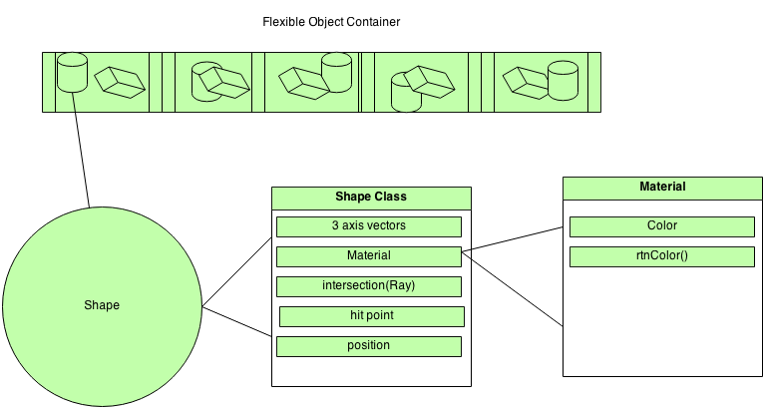
\includegraphics[height=3.0in]{figures/data_structure.png}
\caption{Data structure design for each program}
\label{fig:RayTracerDataStructure}
\end{figure}

It is more difficult to accomplish the data structure task in C++ and Processing (Java).  Just as a variable must be of the same type to save it to a class, all objects must be of the same type to add them to a data structure.  Furthermore, the most basic data structure, an Array, must be declared a specific size upon initialization.  The size issue can be easily circumvented, however.  For each language there is a dynamic container that will grow and shrink in size. C++ has a vector data structure and Processing has an ArrayList. To declare each is simple:
\begin{lstlisting}[language=C++, caption=C++ Vector Example, style=mystyle]
vector <Sphere> sphere_list;
Sphere sphere_object = new Sphere();
sphere_list.push_back(sphere_object);
\end{lstlisting}
\begin{lstlisting}[language=Java, caption=Java ArrayList Example, style=mystyle]
ArrayList<Sphere> sphere_list = new ArrayList<Sphere>();
Sphere sphere_object = new Sphere();
sphere_list.add(sphere_object);
\end{lstlisting}
Each of the above examples creates a \textit{Sphere} list, an instance of a \textit{Sphere} object, and subsequently puts that \textit{Sphere} object into the \textit{Sphere} list.  Note that each structure \textit{must} be declared as the type of object that is being placed into it. The ``pass-by-reference" tactic in C++ is what allows different variable types to be saved to a common parent data structure, as follows:
\begin{lstlisting}[language=C++, caption=C++ Vector Example, style=mystyle]
vector <Shape*> shape_list;
Shape *sphere_object = new Sphere();
Shape *cube_object = new Cube();
shape_list->push_back(sphere_object);
shape_list->push_back(cube_object);
\end{lstlisting}
Declaring the vector with the ``*" denotes a C++ pointer, or that the variable will use the ``pass-by-reference" schema.  Pass-by-reference and pass-by-value variables cannot be combined within a data structure.  To then call any functions within the pointer variables, ``-\textgreater" must be used rather than ``.".  This allows for all shape objects to be saved within the same data structure.

To accomplish this in Processing the Shape class was declared as abstract in Figure \ref{list:javaClass}.  This keyword signifies that an object of this type may not be instantiated within a program.  This keyword demonstrates true inheritance because it acts as a placeholder for commonly used functions and variables between class types.  In Java, it allows child classes to be declared as common types without losing each class's individual functions and variables. This is accomplished as follows:
\begin{lstlisting}[language=Java, caption=Java ArrayList Example, style=mystyle]
ArrayList<Shape> shape_list = new ArrayList<Shape>();
Shape sphere_object = new Sphere();
Shape cube_object = new Cube();
shape_list.add(sphere_object);
shape_list.add(cube_object);
\end{lstlisting}
\doublespacing
Notice that sphere\_object and cube\_object are declared as a type shape but using the child class's individual constructors.  This allows ``shape\_list.add()" to be called on the next two lines without throwing an error.  If the Shape class was not declared as abstract, when declaring Shape sphere\_object and calling the child constructor, and when calling functions that are specific to the child class, those calls will be replaced with calls to the parent class's functions.  

While Java still has ``pass-by-value" and ``pass-by-reference", Processing/Java has simplified their language to effectively make all declared variables function as pointers, pointing back to the original variable declaration.

\subsection{Python Inheritance and Data Structures}
While parent classes are not important for Python list functionality because Python is considered a dynamically-typed language (as opposed to the static-type for C++ and Java), for organizational purposes they were used and inheritance was declared as follows (note tabs and spacing), using the same example:

\singlespacing
\begin{lstlisting}[language=Python, style=mystyle]
//shape.py file//
class Shape(object):
    __init__(self,...):
        //shape constructor
    def size(self,...):
        //size calculation for all child classes
\end{lstlisting}
\begin{lstlisting}[language=Python, caption=Python Class Inheritance Example, style=mystyle]
//sphere.py file//
import Shape
class Sphere(Shape.Shape):
    def __init__(self,...):
        //sphere constructor contents
    def size():
        //calculate size specific for sphere
\end{lstlisting}
\begin{center}
\line(1,0){100}
\end{center}
\doublespacing
\subsubsection{Data Structure}
Accomplishing the data structure task in Python is the most simple and takes no extra effort.  Simply declare an object and place it in a Python list, like so:
\begin{lstlisting}[language=Python, caption=Python List Example, style=mystyle]
sphere = Sphere.Sphere();
cube = Cube.Cube();
objects =  [];
objects.append(sphere);
objects.append(cube);
\end{lstlisting}
The above code creates a sphere object, cube object, and an objects list, then adds the sphere and cube into the data structure with the lists append method.  Python lists can accept any combination of different variable types, which can be useful for a ray-tracers implementation but dangerous for software prosperity and robustness.  If the assumption is that all variables in a list have the same type and therefore the same associated functions, when an object that does not fall under these assumptions gets added to the list the program will fail.  More care needs to be taken to make sure all variables are of the correct type that are added to a list to ensure that the program will run successfully, since this is not required for the program to initially start running.

\subsection{Milestone Results: Processing Time Overview and Images}
Once the issues with class and object declaration were solved implementing the Basic Ray Casting Milestone was very straightforward with each language.  There was one issue with the Processing language, however, that accounted for a majority of the Processing implementation and accounts for a core theory of ray tracing implementation.
\subsubsection{Left Hand vs. Right Hand Rule}
In the 3-D virtual world there is a set of governing rules that determine an object's position within the space, known as a coordinate plane.  As in a two dimensional graph, a 3D scene contains an X and Y coordinate, but a new coordinate, Z, is added.  The order and direction for each of these axes, as they're called, determines many important calculations when determining size and space of objects in the scene.  Left-handed and right-handed can be described as follows(from processing.org):

\begin{quote}
``In order to draw something at a point in three dimensions the coordinates are specified in the order you would expect: x, y, z. Cartesian 3D systems are often described as ``left-handed" or ``right-handed." If you point your index finger in the positive y direction (up) and your thumb in the positive x direction (to the right), the rest of your fingers will point towards the positive z direction. It's left-handed if you use your left hand and do the same."
\end{quote}
For the C++ and Python implementations of the ray tracers a coordinate system needed to be created from scratch. I am right handed and therefore a right-handed coordinate system was used.  This means, when looking at a computer monitor, the positive Y axis points towards the top of the screen, the positive X axis points to the right of the screen and the negative Z axis points directly out of the screen, perpendicular to the screen's surface.  This is not a typically traditional schema for coordinate planes with computers, nor is it the scheme used by Processing.  Processing used a left-handed coordinate system where the positive y axis points towards the bottom of the screen, the positive X axis points towards the right of the screen, and the positive Z points away from the user, towards the back of the computer, perpendicular with the computer screen.  Many of the calculations associated with cross products and other vector math needed the Y value and Z value negated so that the caluclations behaved more similarly to the other two ray tracing programs.
\subsection{Basic Ray Casting Images}
Here are a few images from the Basic Ray Casting Milestone.  While these are just a few examples from each language and each task, each language accomplished the same types of images that are presented in Figures \ref{fig:processingraycasting} through \ref{fig:processingtriangles}.
\begin{figure}[ht]
\centering
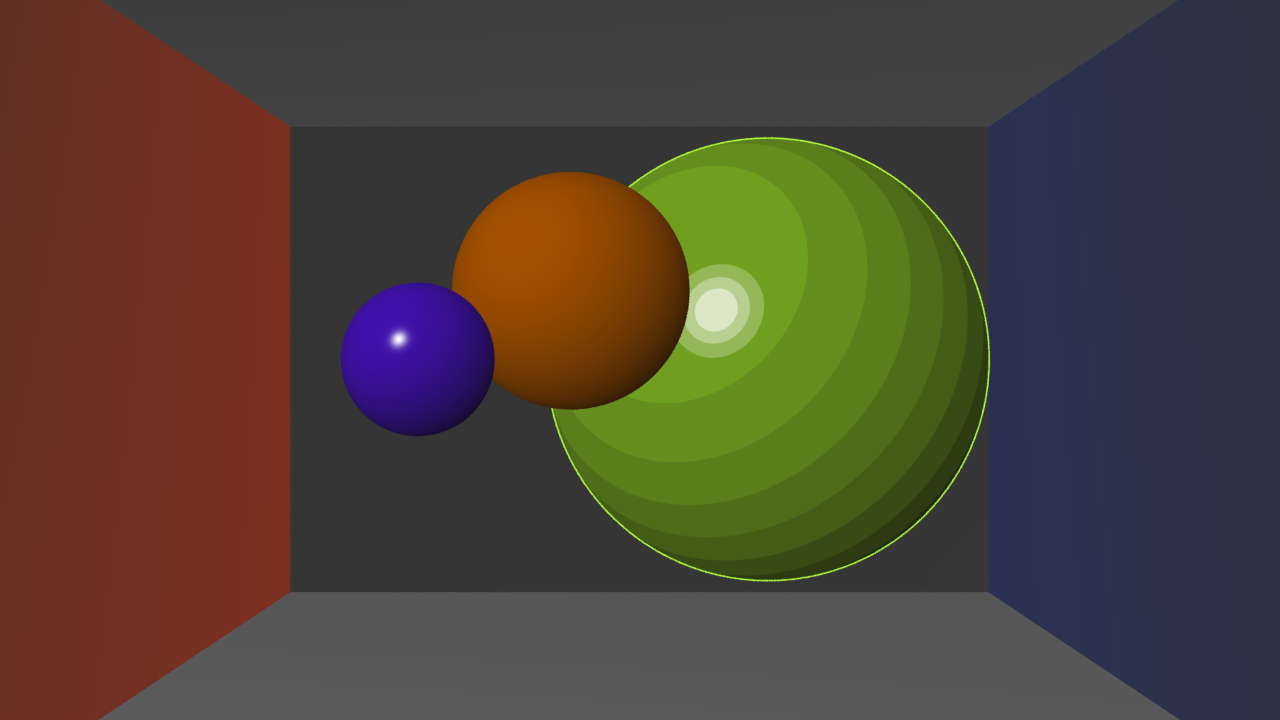
\includegraphics[width=\textwidth]{figures/BasicRayCastingProcessing.png}
\caption{Ray Casting Accomplished with Processing. Shown are three spheres with a different texture type for each, and five planes all with flat textures applied.}
\label{fig:processingraycasting}
\end{figure}

\begin{figure}[ht]
\centering
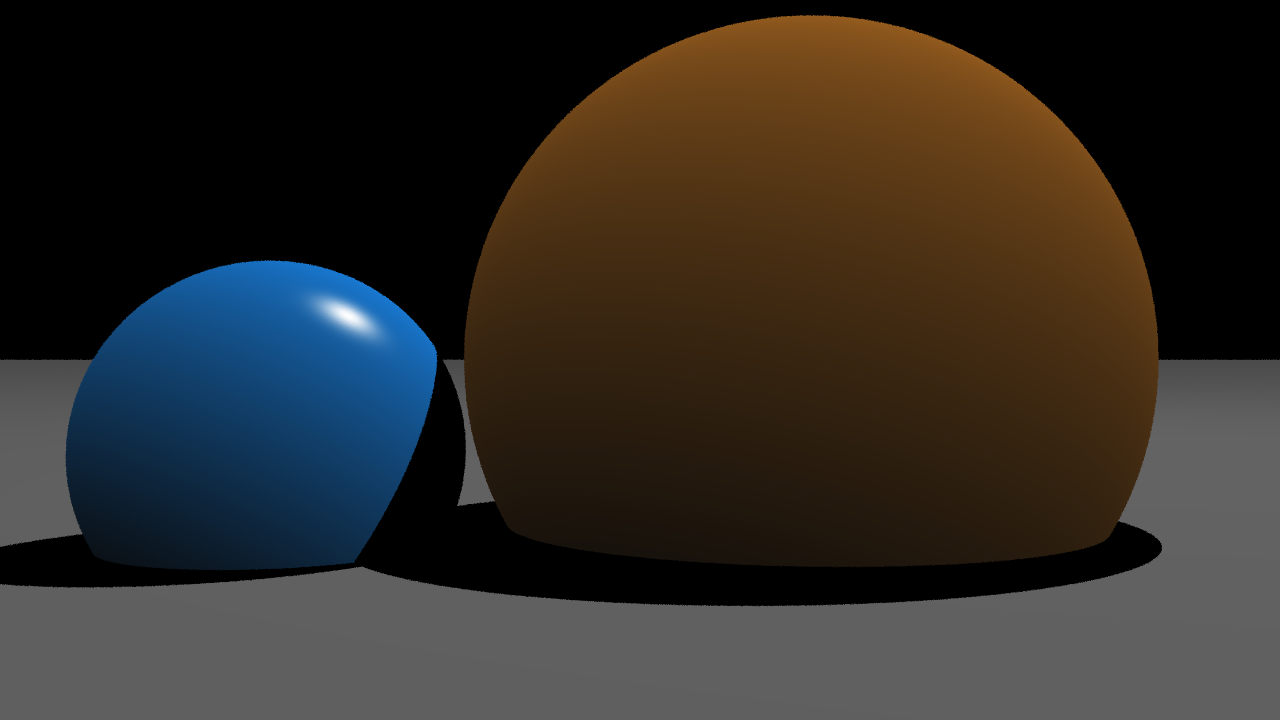
\includegraphics[width=\textwidth]{figures/ShadowCastingPython.png}
\caption{Ray Casting Accomplished with Python.  Shown are two spheres, and one plane that all cast shadows from a simple point light. }
\label{fig:pythonraycasting}
\end{figure}

\begin{figure}[ht]
\centering
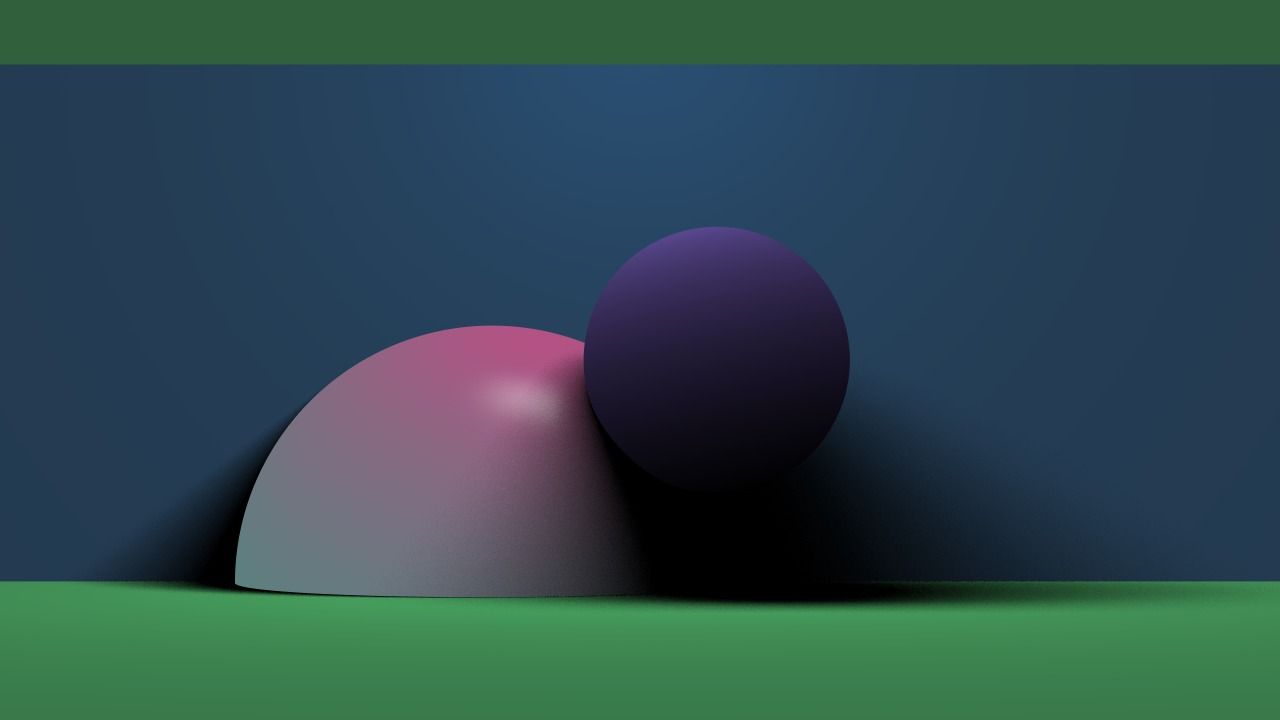
\includegraphics[width=\textwidth]{figures/ShadowCastingC++.jpeg}
\caption{Ray Casting Accomplished with C++.  Shown are two spheres, five planes and an area light that all cast shadows, which accounts for the soft shadow effect. }
\label{fig:cplusraycasting}
\end{figure}

\begin{figure}[ht]
\centering
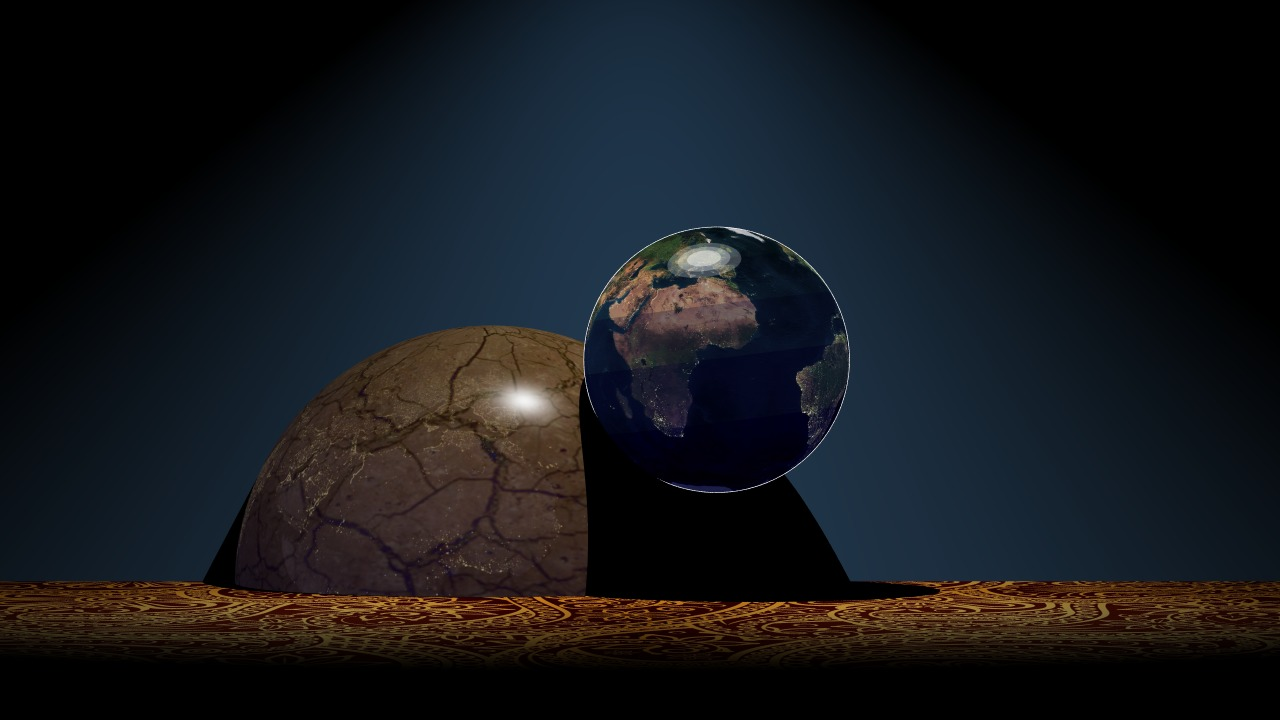
\includegraphics[width=\textwidth]{figures/texturingC++.jpg}
\caption{Ray Casting Accomplished with C++.  Shown are two spheres with 2 separate shader types with two separate images mapped to them, and two planes, one with a repeated image texture and one without any image texture. }
\label{fig:cplusraycasting}
\end{figure}

\begin{figure}[ht]
\centering
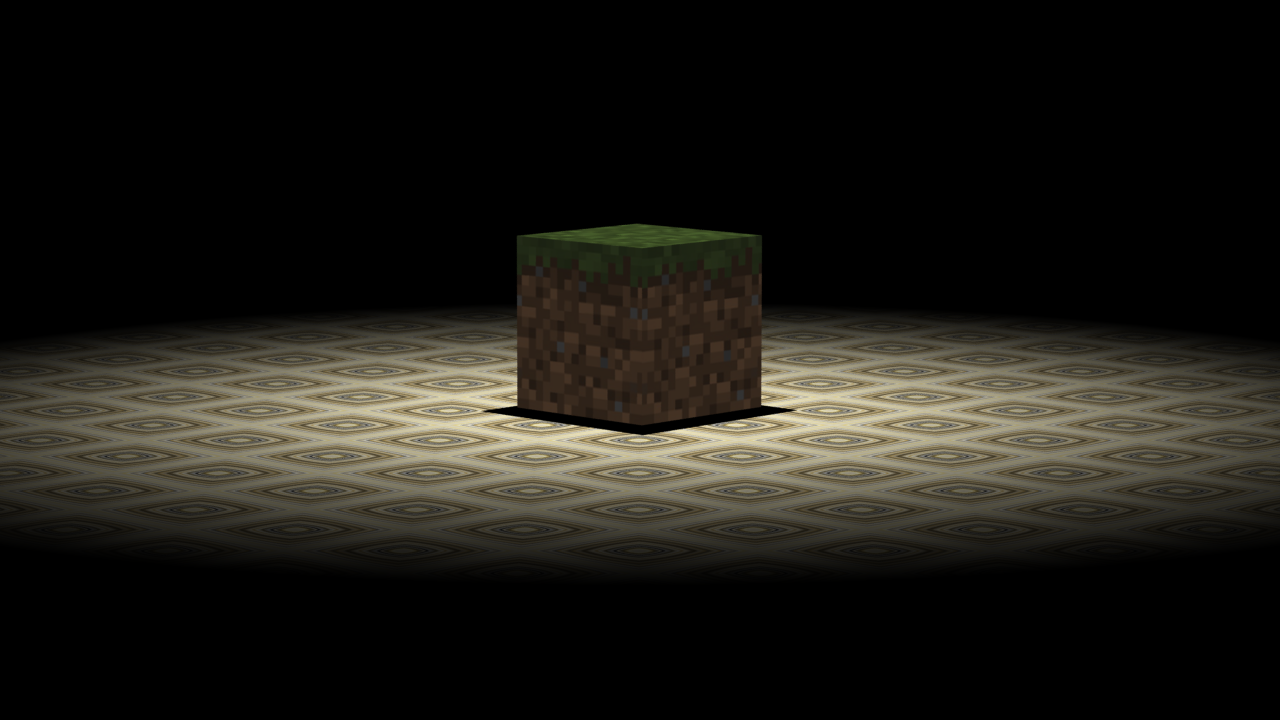
\includegraphics[width=\textwidth]{figures/processingTriangles.png}
\caption{Ray Casting Accomplished with Processing. One cube with twelve triangles and an image mapped to it on a plane with a repeated image texture illuminated by a spotlight.}
\label{fig:processingtriangles}
\end{figure}

\subsection{Performance Results}
For each test in Basic Ray Casting a variety of levels of complexity were tested in order to see how each language handles a different amount of load.  For each rendering a 1280 x 720 image size was used to generate a high quality image for testing.  The results are graphed and labeled in Figures \ref{fig:basicgraph} - \ref{fig:texgraph}.
\begin{figure}[ht]
\centering
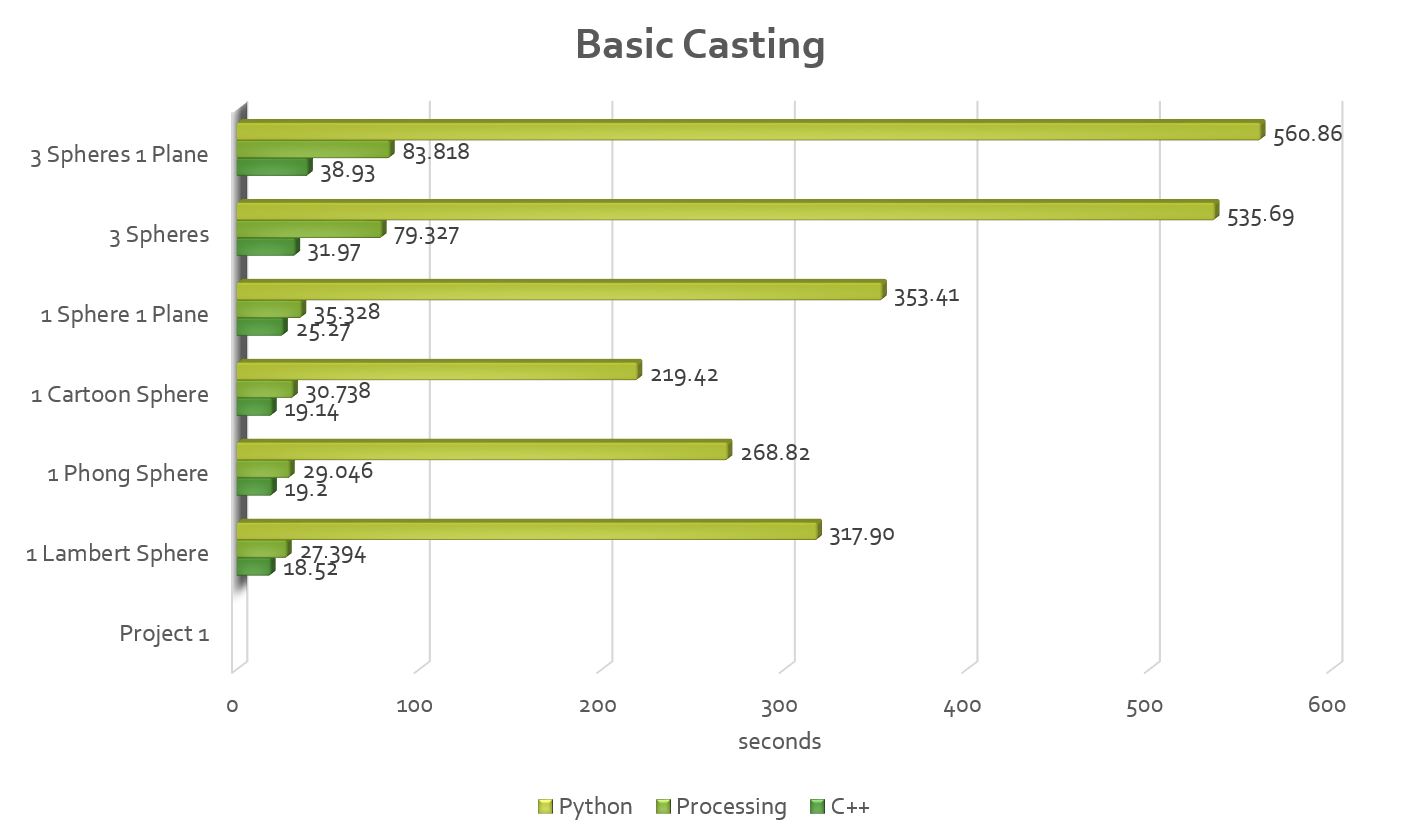
\includegraphics[width=\textwidth]{figures/graphs/basic-graph.png}
\caption{Basic ray tracing performance graph for each language}
\label{fig:basicgraph}
\end{figure}

\begin{figure}[ht]
\centering
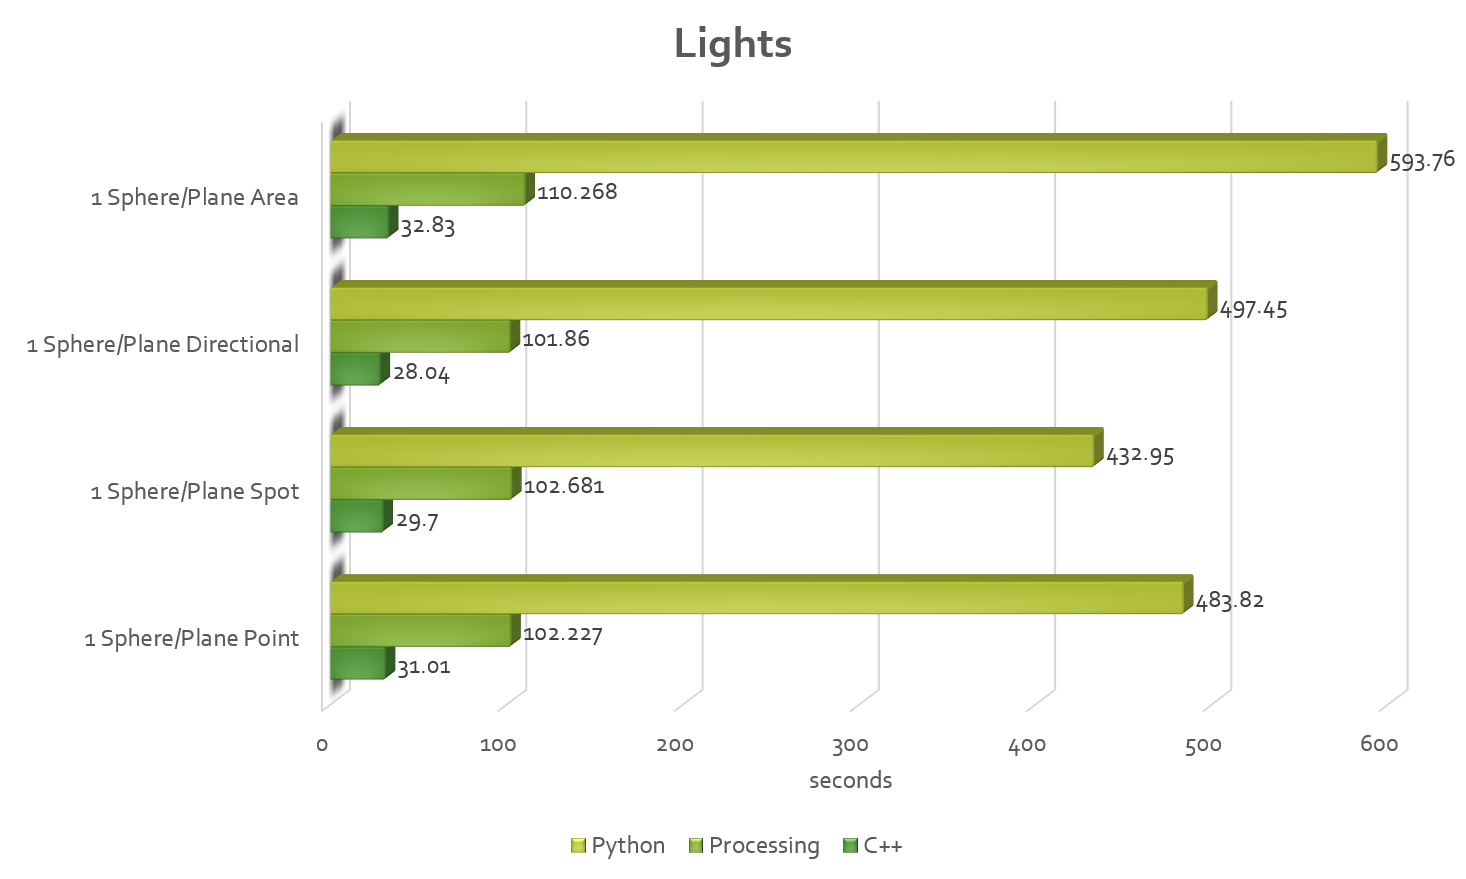
\includegraphics[width=\textwidth]{figures/graphs/lights-graph.png}
\caption{Light's performance graph for each language}
\label{fig:lightsgraph}
\end{figure}

\begin{figure}[ht]
\centering
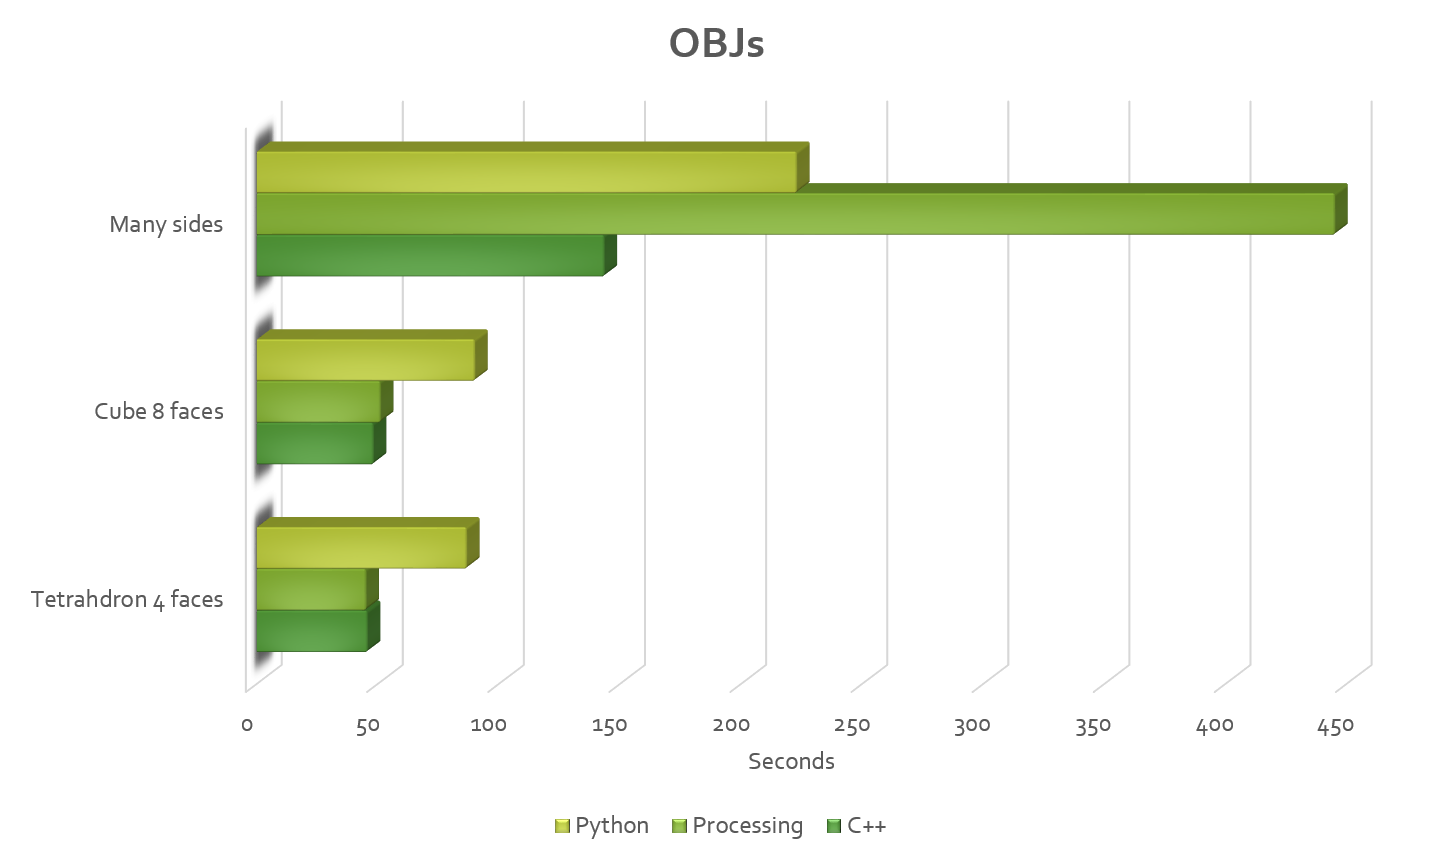
\includegraphics[width=\textwidth]{figures/graphs/obj-graph.png}
\caption{OBJ Performance Graph for each language}
\label{fig:objgraph}
\end{figure}

\begin{figure}[ht]
\centering
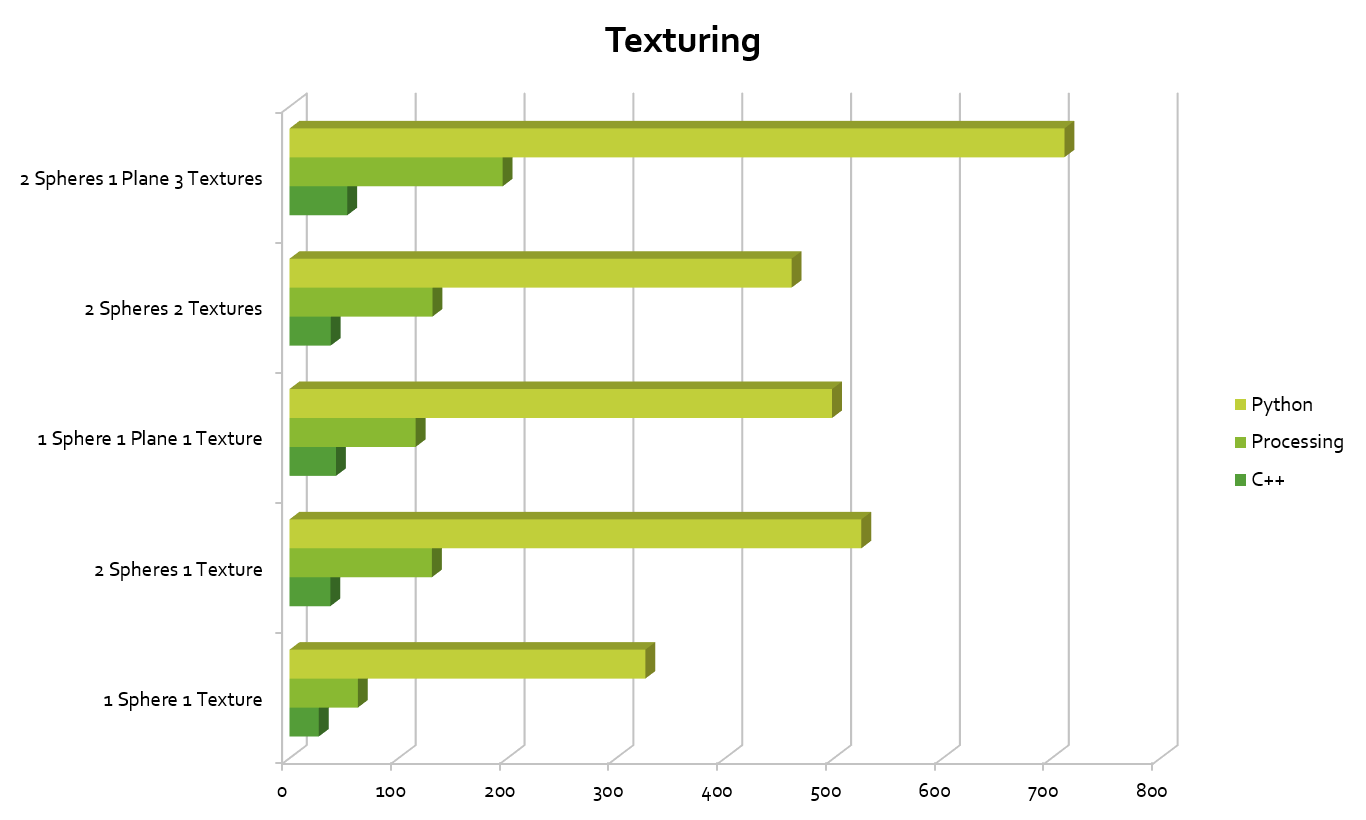
\includegraphics[width=\textwidth]{figures/graphs/texturing.png}
\caption{Texturing Performance Graph for each language}
\label{fig:texgraph}
\end{figure}

%%%%%%%%%%%%%%%%%%%%%%%%%%%%%%%%%%%%%%%%%%%%%%%%%%%%%%
%%%%%%%%%%%%%%%%%%%%%%%%%%%%%%%%%%%%%%%%%%%%%%%%%%%%%%
\section{Milestone 3: Ray Tracing and Distributed Ray Tracing}
The main complications discovered for this milestone where all related to the implementation of a recursive ray tracing strategy.  All three languages had the same difficulties that were not unique to each implementation.  To implement recursion requires the knowledge of establishing a process function within each raytracing function that will repeatedly call itself unless specific escape conditions are met.  It is important to establish these conditions such that they are met within the execution of the program or else the ray tracer will implement an infinite loop that will consume computing resources until the computer crashes and needs to be restarted.

The main challenge introduced for distributed ray tracing was the idea of randomness.  In order to get a jitter for every vector value for some aspect of the ray tracing process, whether it be the hit point or the view point of the camera.  To achieve this effect was different in each language, but Processing and Python were surprisingly similar.

\singlespacing
\begin{lstlisting}[language=C++, caption=C++ Random Function, style=mystyle, label=c++Rand]
float randNum(float LO, float HI)
{
    float U2 = LO + (float)rand()/((float)RAND_MAX/(HI-LO));
    return U2;
}
\end{lstlisting}
\begin{lstlisting}[language=Java, caption=Processing Random Function, style=mystyle, label=processingRand]
random(0.0,1.0);
\end{lstlisting}
\begin{lstlisting}[language=Python, caption=Python Random Function, style=mystyle, label=pythonRand]
random.uniform(0.0,1.0);
\end{lstlisting}
\doublespacing

Processing and Python each had their own random libraries that handled generating random numbers between two specified values but in C++ it was not provided.  Writing a random function took a lot of overhead and wasted time comprehending how computers generate random numbers in C++ at a foundational level.  It was significantly easier and more intuitive to implement a random function in both Python and Processing than it was in C++.

\subsection{Ray Tracing and Distributed Ray Tracing Images}
Here are a few images from the Ray Tracing and Distributed Ray Tracing Milestone.  While these are just a few examples from each language and each task, each language accomplished the same types of images that are presented in Figures \ref{fig:pyFlect} through \ref{fig:pyDist}.

\begin{figure}[ht]
\centering
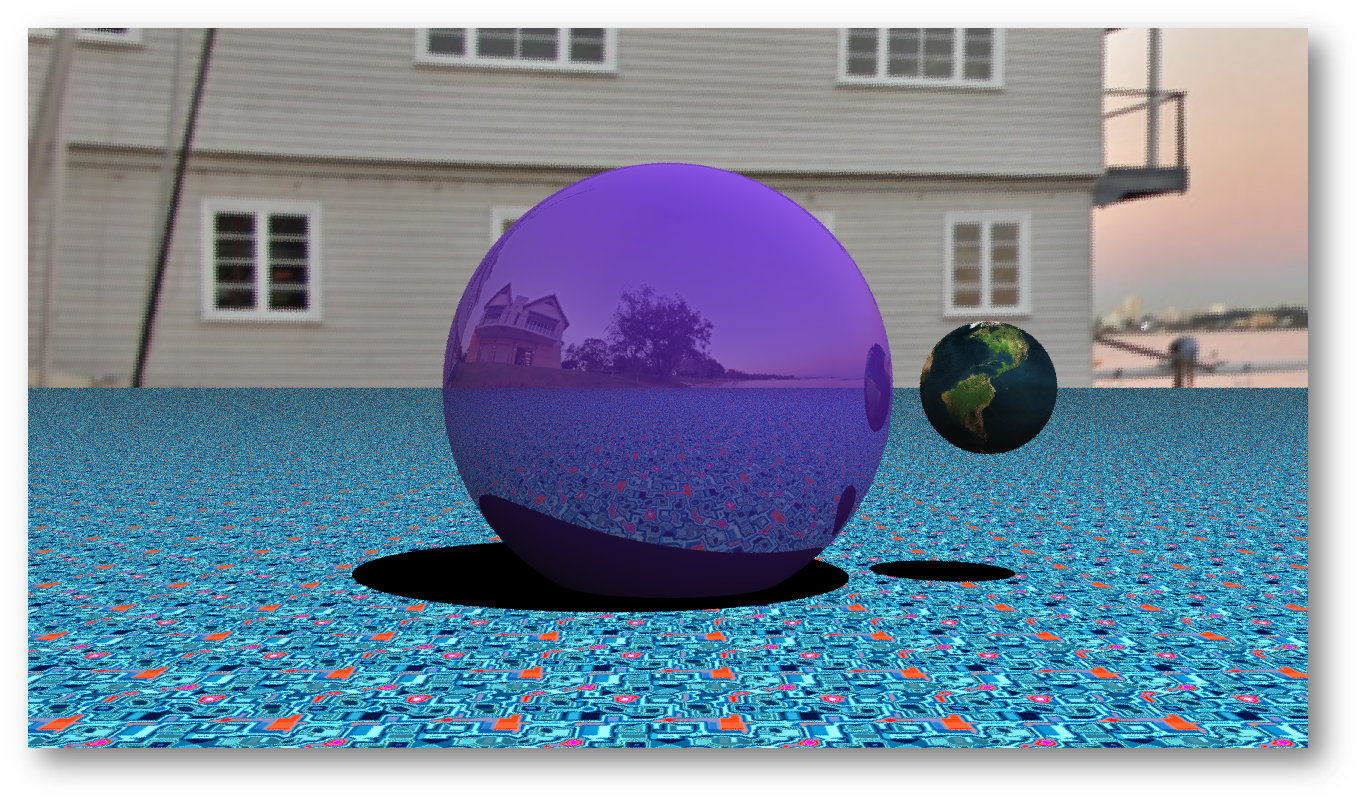
\includegraphics[width=\textwidth]{figures/python-reflection.png}
\caption{Reflection effect completed in Python}
\label{fig:pyFlect}
\end{figure}
\begin{figure}[ht]
\centering
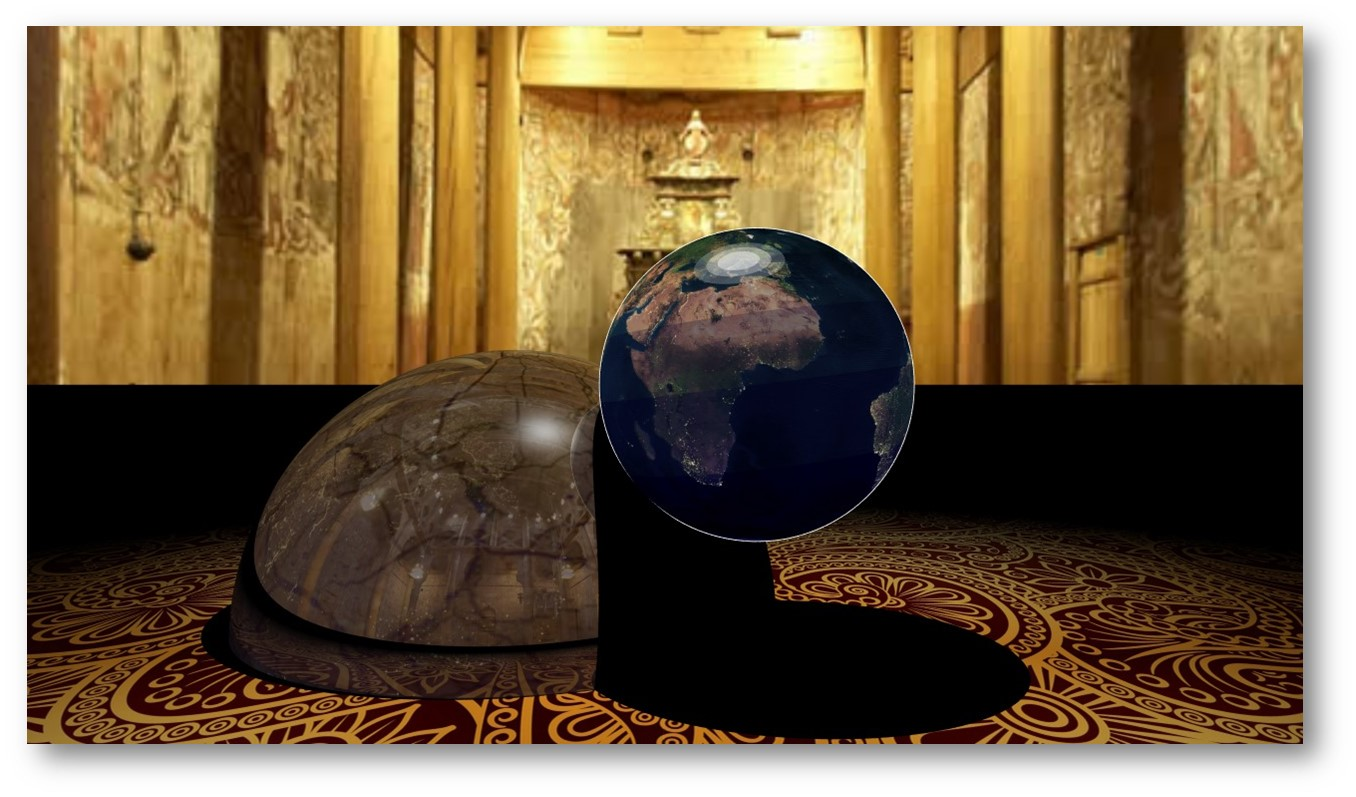
\includegraphics[width=\textwidth]{figures/c++-reflective.jpg}
\caption{Reflection Effect completed with C++}
\label{fig:c++Flect}
\end{figure}
\begin{figure}[ht]
\centering
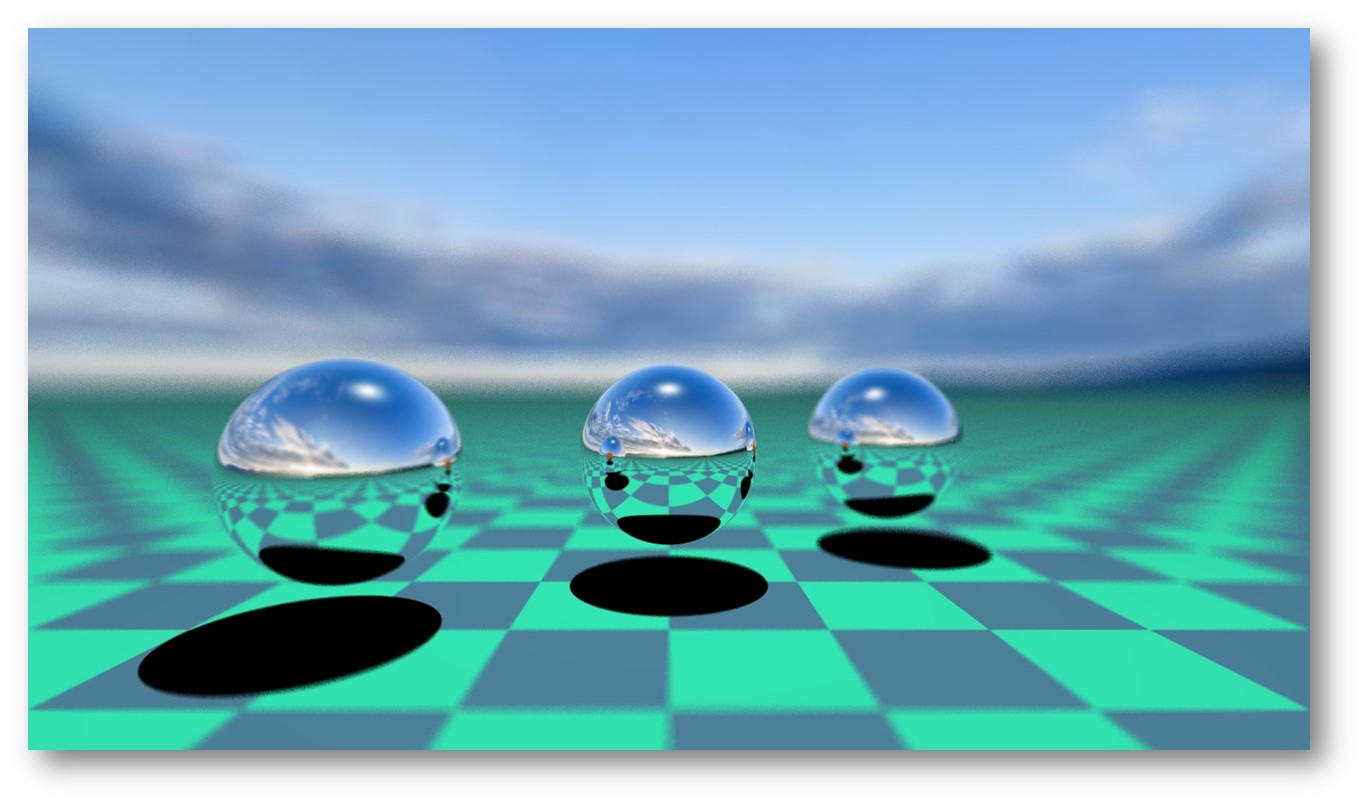
\includegraphics[width=\textwidth]{figures/c++-distributed.jpg}
\caption{Depth of Field effect captured with C++}
\label{fig:c++Dist}
\end{figure}
\begin{figure}[ht]
\centering
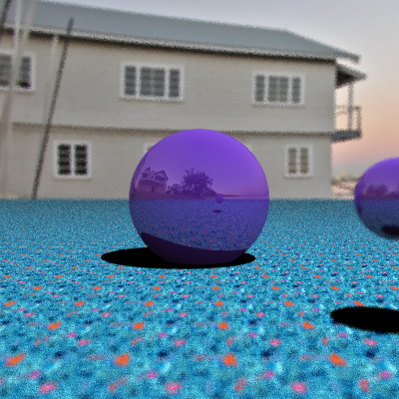
\includegraphics[width=300px]{figures/python-distributed.png}
\caption{Depth of Field effect captured with Python.  Pixelated image shows one of the restrictions of Python computing power for an image of this scale.}
\label{fig:pyDist}
\end{figure}

\subsection{Performance Results}
Performance results each language can be seen in Figure \ref{refGraph}
\begin{figure}[ht]
\centering
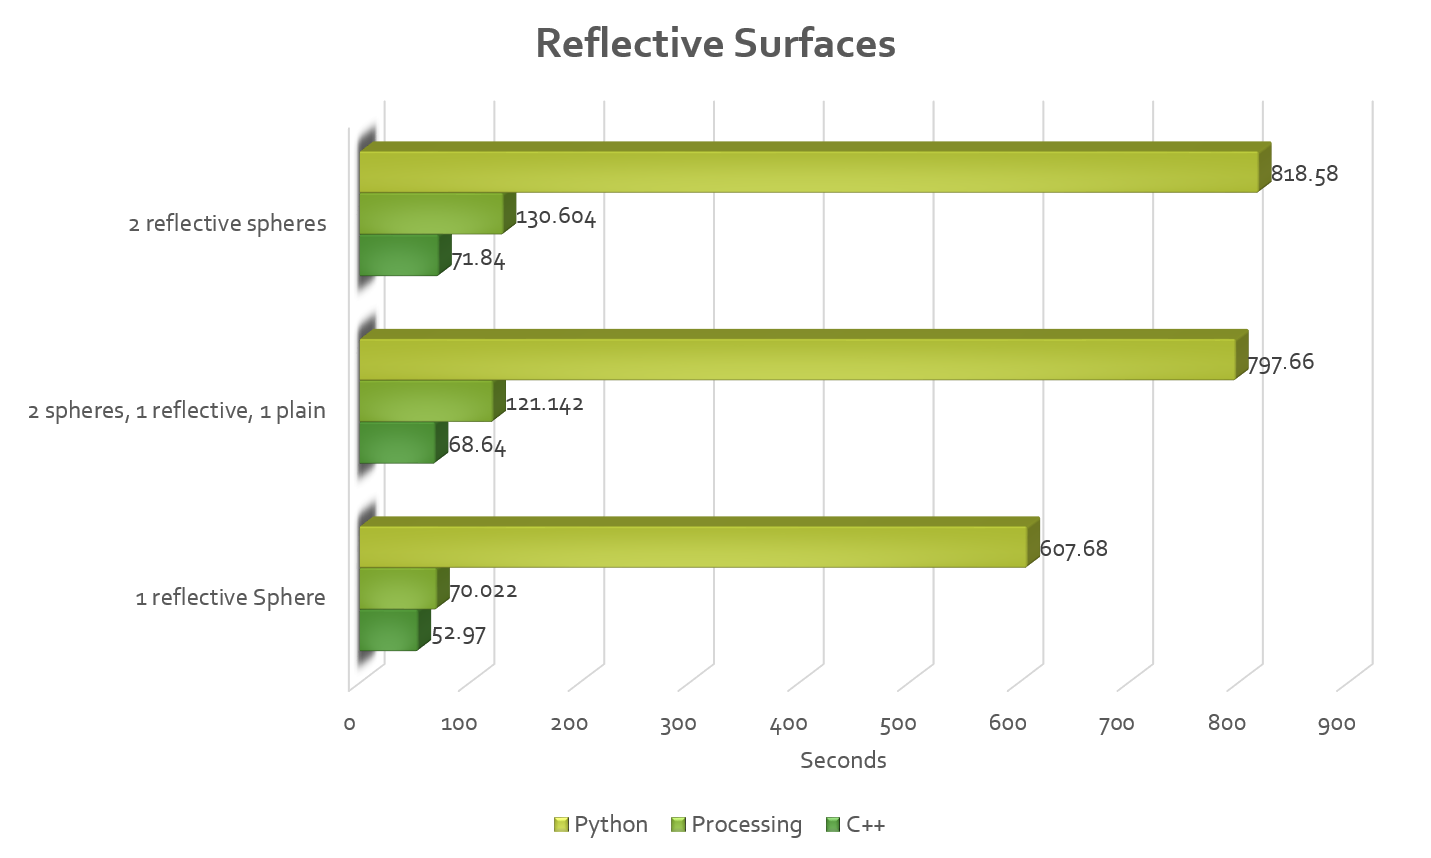
\includegraphics[width=\textwidth]{figures/graphs/reflective-graph.png}
\caption{Texturing Performance Graph for each language}
\label{fig:refGraph}
\end{figure}

\section{Milestone 4: Indirect Illumination}
Milestone 4 experienced the same complications as Milestone 3, with the majority of the implementation being the same throughout all three languages.  No new computer science concepts were introduced for this section, so this Milestone was completely based upon ray tracing theory rather than language implementation.  By this time I had fully mastered the languages and felt comfortable accomplishing the tasks in each.
\subsection{Indirect Illumination Images}
Images for the Indirect Illumintaion Milestone can be found in Figure \ref{fig:c++AO}.
\begin{figure}[ht]
\centering
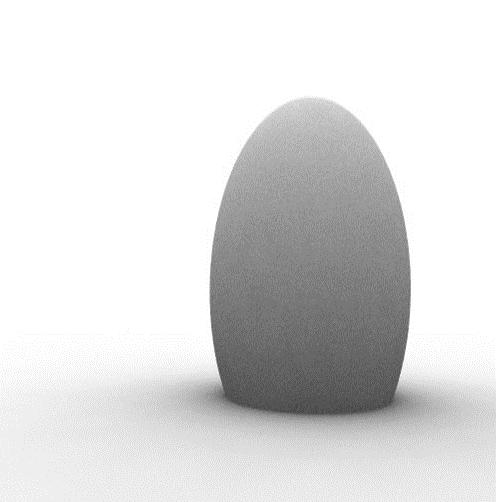
\includegraphics[width=\textwidth]{figures/indirectIllumination-c++.png}
\caption{Ambient Occlusion effect created with C++}
\label{fig:c++AO}
\end{figure}

%%%%%%%%%%%%%%%%%%%%%%%%%%%%%%%%%%%%%%%%%%%%%%%%%%%
%
%  New template code for TAMU Theses and Dissertations starting Fall 2012.
%  For more info about this template or the
%  TAMU LaTeX User's Group, see http://www.howdy.me/.
%
%  Author: Wendy Lynn Turner
%	 Version 1.0
%  Last updated 8/5/2012
%
%%%%%%%%%%%%%%%%%%%%%%%%%%%%%%%%%%%%%%%%%%%%%%%%%%%
%%%%%%%%%%%%%%%%%%%%%%%%%%%%%%%%%%%%%%%%%%%%%%%%%%%%%%%%%%%%%%%%%%%%%%
%%                           SECTION III
%%%%%%%%%%%%%%%%%%%%%%%%%%%%%%%%%%%%%%%%%%%%%%%%%%%%%%%%%%%%%%%%%%%%%


\chapter{\uppercase{Results and Conclusions}}

Each language had it's own advantages and disadvantages to the ray tracing process.  These were further accentuated by the speed tests conducted for each Milestone.  The results for each speed test were to be as expected from common knowledge of each language, and from more rigorous tests conducted by other computer scientists.  Python was the slowest by far, with Processing holding the middle ground and C++ being the fastest.  Surprisingly however, the speed difference between Processing and C++ is less than what might have been expected, since C++ is compiled before running the test and Processing's speed test is considered with the processing ``play'' button, which assumedly compiles and runs the code all at once.  

\section{Conclusions}
Each language will be discussed with it's pro's and con's and at the end of this section a recommendation will be made as to the most suitable language that might maximize focus on the implementation theory rather than the implementation process of writing code syntax.  It can be established as a baseline for all languages however that you MUST learn a certain baseline of scripting and coding concepts. Language syntax and compilation processes cannot be avoided.  

\subsection{C++}
C++ is the fastest processor of all the languages tested.  This allowed for quicker iterations and more creative freedom with the final images because of the speed.  C++ was able to process the scale of computation for large images far quicker that either Java or Python.  However, C++ is not an easy language to learn.  There was much more overhead to learn in order to compile and set up an C++ project.  Whereas in the other languages you just needed to learn how to create a executable file and run that within the correct environment, C++ had a variety of compilers to choose from, and then a multitude of files and commands to run before the image would appear on the screen.  This could be automated to save time, but the initial process to a new programmer is not intuitive to quickly write and execute a ray tracer.  However, having written the first ray tracer in C++, which exposes the basic process of how a computer handles executing a program, since with C++ you need to ``make'' and then run the program, this intuitively allowed the implementation of the other ray tracers to go faster.  However, since practically most artists will be writing only one ray tracer, the knowledge of how to compile and run the program still needs to be accomplished, but is less forgiving or intuitive with C++.  C++ error handling is uninformative to the untrained programmer, giving responses like %TODO ADD C++ ERRORS HERE%%

\subsection{Processing}
Processing was the easiest to compile and execute code.  Processing has expedited this process by packaging the code compiler within it's own custom ``API'' (processing the language for this thesis encompasses both the java language and the processing executable that is delivered with a download of Processing).  While Processing comes with a the necessary libraries to implement a ray tracer, using these introduces another challenge.  Addition in this language with the supplied Vector form was done through a function(Vector.add()) rather than through an operator (such as plus ``+'' or minus ``-'').  While unintuitive for complex math functions, over all this was a small setback in creating a raytracer.  The benefits of an expedited compilation process out weighs the initial difficulty of figuring out language syntax.  Error handling in Processing is more informative as well, and will bring you to the section of the code where the error occurred.  This is a benefit of using the Processing IDE as a part of the processing language, which does not happen when receiving an error from python or C++.

\subsection{Python}
Python was the slowest of all the languages test.  However, it was the easiest to write code in.  By design it strives to have the most intuitive syntax of all the languages.  While there are still rules to follow when creating Python code, as there are in C++ or in Processing, there are far less of them.  Python however still needed the use of include statements, which can be a difficult concept to grasp when writing large programs. Since Java and C++ are both statically typed, they need more strict rules as to when variables can be set and what those variables can be set as.  A lot of time was spent learning and understanding polymorphism and sub-typing for Java and C++ so that each ray tracer can more closely mimic the ray tracing theory.  With Python, none of this research was necessary in order to accomplish these complex data structures.  However Python was significantly slower than both Python and Processing.  While this means Pixar or Dreamworks will not be using Python for their next iteration of their ray tracer, for learning ray tracing theory this was of no consequence.  When establishing a workflow to create a python image, a lower resolution ``layout'' was used to prepare a final render, instead of testing images with the full resolution every time.  Though it's biggest set back was speed, work arounds could be implemented to allow for a speedier artistic development process.  For single frame rendering, five minutes is not a long time to wait for the final product.  To iterate over artistic versions of a rendered image, a lower resolution image that only takes 30 seconds can be used instead.  The final image only needs to be the final resolution, and therefore take the full five minutes.

\section{Final Recommendation}
For every language you need to learn computer science terms like classes and recursion.  This is beneficial to the overall process and cannot be avoided.  In addition, it is understood that in each language there is a necessary evil of learning some sort of syntax related information.  Every language has it's own quirks, and these quirks make the respective language that much easier or more difficult to use.  The learning time for each language to process syntax and data types was relatively equal for each language.  Therefore the deciding limiting factor that this recommendation is based off of is the set-up overheard that is required to learn before any code is written.  Processing is the best recommendation in this regard.  While Processing has some unintuitive syntax, learning that syntax takes no more time than learning the syntax of C++ or Python, and probably takes less time the the total time taken to learn how to set-up Python and C++ in whatever environment you're developing in.  While with C++ you must understand make files and header files once the code has even installed, Processing has packaged all this overhead into a simple IDE that does the bulk of the work for you.  Processing's compilation times were not drastically  as slow as Python, but when compared to C++ the times do not discredit the language from quick, interactive artistic repetition to achieve the best results.  


%%%%%%%%%%%%%%%%%%%%%%%%%%%%%%%%%%%%%%%%%%%%%%%%%%%%%%%%%%%%%
\let\oldbibitem\bibitem
\renewcommand{\bibitem}{\setlength{\itemsep}{0pt}\oldbibitem}
%%%%%%%%%%%%%%%%%%%%%%%%%%%%%%%%%%%%%%%%%%%%%%%%%%%%%%%%%%%%%%%
%%%%%%%%%%%%%%%%%%%%%%%%%%%%%%%%%%%%%%%%%%%%%%%%%%%
%
%  New template code for TAMU Theses and Dissertations starting Fall 2012.  
%  For more info about this template or the 
%  TAMU LaTeX User's Group, see http://www.howdy.me/.
%
%  Author: Wendy Lynn Turner 
%	 Version 1.0 
%  Last updated 8/5/2012
%
%%%%%%%%%%%%%%%%%%%%%%%%%%%%%%%%%%%%%%%%%%%%%%%%%%%


%%%%%%%%%%%%%%%%%%%%%%%%%%%%%%%%%%%%%%%%%%%%%%%%%%%%%%%%%%%%%%%%%%%%%%
%%                           REFERENCES 
%%%%%%%%%%%%%%%%%%%%%%%%%%%%%%%%%%%%%%%%%%%%%%%%%%%%%%%%%%%%%%%%%%%%%

\phantomsection
\addcontentsline{toc}{chapter}{REFERENCES}

\renewcommand{\bibname}{{\normalsize\rm REFERENCES}}

\bibliographystyle{plain}
\bibliography{references}
% %%%%%%%%%%%%%%%%%%%%%%%%%%%%%%%%%%%%%%%%%%%%%%%%%%%
%
%  New template code for TAMU Theses and Dissertations starting Fall 2012.  
%  For more info about this template or the 
%  TAMU LaTeX User's Group, see http://www.howdy.me/.
%
%  Author: Wendy Lynn Turner 
%	 Version 1.0 
%  Last updated 8/5/2012
%
%%%%%%%%%%%%%%%%%%%%%%%%%%%%%%%%%%%%%%%%%%%%%%%%%%%

\begin{appendices}
\titleformat{\chapter}{\centering\normalsize}{APPENDIX \thechapter}{0em}{\vskip .5\baselineskip\centering}
\renewcommand{\appendixname}{APPENDIX}

%%%%%%%%%%%%%%%%%%%%%%%%%%%%%%%%%%%%%%%%%%%%%%%%%%%
%
%  New template code for TAMU Theses and Dissertations starting Fall 2012.  
%  For more info about this template or the 
%  TAMU LaTeX User's Group, see http://www.howdy.me/.
%
%  Author: Wendy Lynn Turner 
%	 Version 1.0 
%  Last updated 8/5/2012
%
%%%%%%%%%%%%%%%%%%%%%%%%%%%%%%%%%%%%%%%%%%%%%%%%%%%

%%%%%%%%%%%%%%%%%%%%%%%%%%%%%%%%%%%%%%%%%%%%%%%%%%%%%%%%%%%%%%%%%%%%%%
%%                           APPENDIX A 
%%%%%%%%%%%%%%%%%%%%%%%%%%%%%%%%%%%%%%%%%%%%%%%%%%%%%%%%%%%%%%%%%%%%%

\phantomsection

\chapter{\uppercase{First Appendix}}

Text for the Appendix follows.

\begin{figure}[H]
\centering
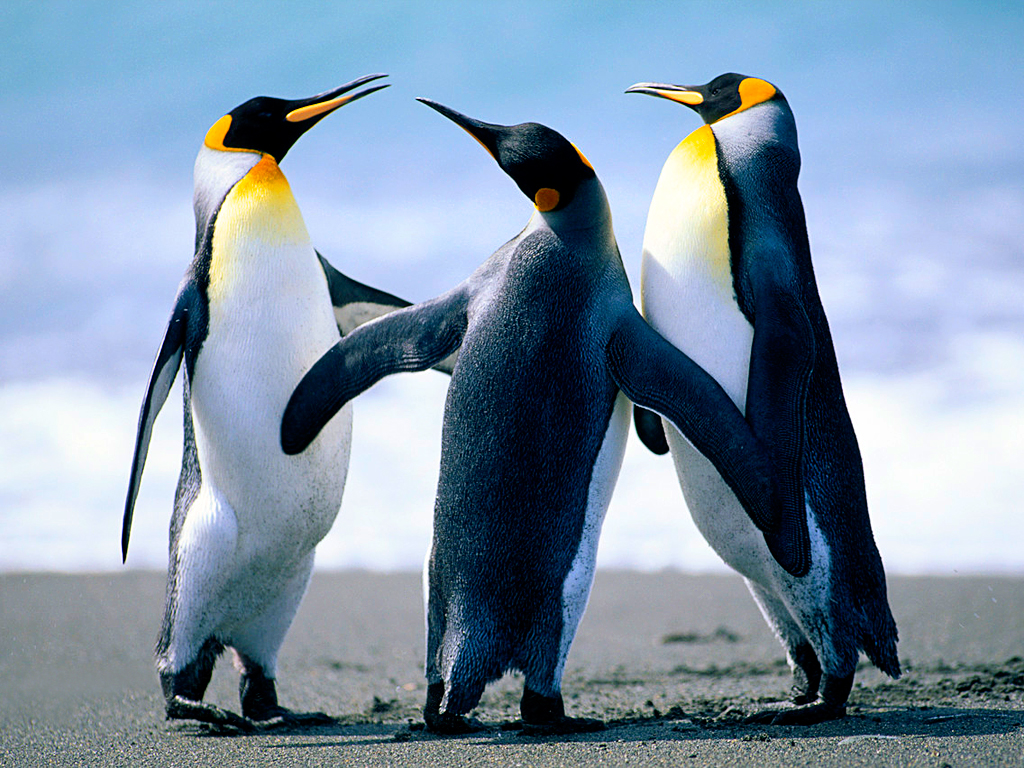
\includegraphics[scale=.50]{figures/Penguins.jpg}
\caption{TAMU figure}
\label{fig:tamu-fig5}
\end{figure}

%%%%%%%%%%%%%%%%%%%%%%%%%%%%%%%%%%%%%%%%%%%%%%%%%%%
%
%  New template code for TAMU Theses and Dissertations starting Fall 2012.  
%  For more info about this template or the 
%  TAMU LaTeX User's Group, see http://www.howdy.me/.
%
%  Author: Wendy Lynn Turner 
%	 Version 1.0 
%  Last updated 8/5/2012
%
%%%%%%%%%%%%%%%%%%%%%%%%%%%%%%%%%%%%%%%%%%%%%%%%%%%

%%%%%%%%%%%%%%%%%%%%%%%%%%%%%%%%%%%%%%%%%%%%%%%%%%%%%%%%%%%%%%%%%%%%%%
%%                           APPENDIX B
%%%%%%%%%%%%%%%%%%%%%%%%%%%%%%%%%%%%%%%%%%%%%%%%%%%%%%%%%%%%%%%%%%%%%

\chapter{\uppercase {Second Appendix with a longer title - much longer in fact}}

Text for the Appendix follows.

\begin{figure}[H]
\centering
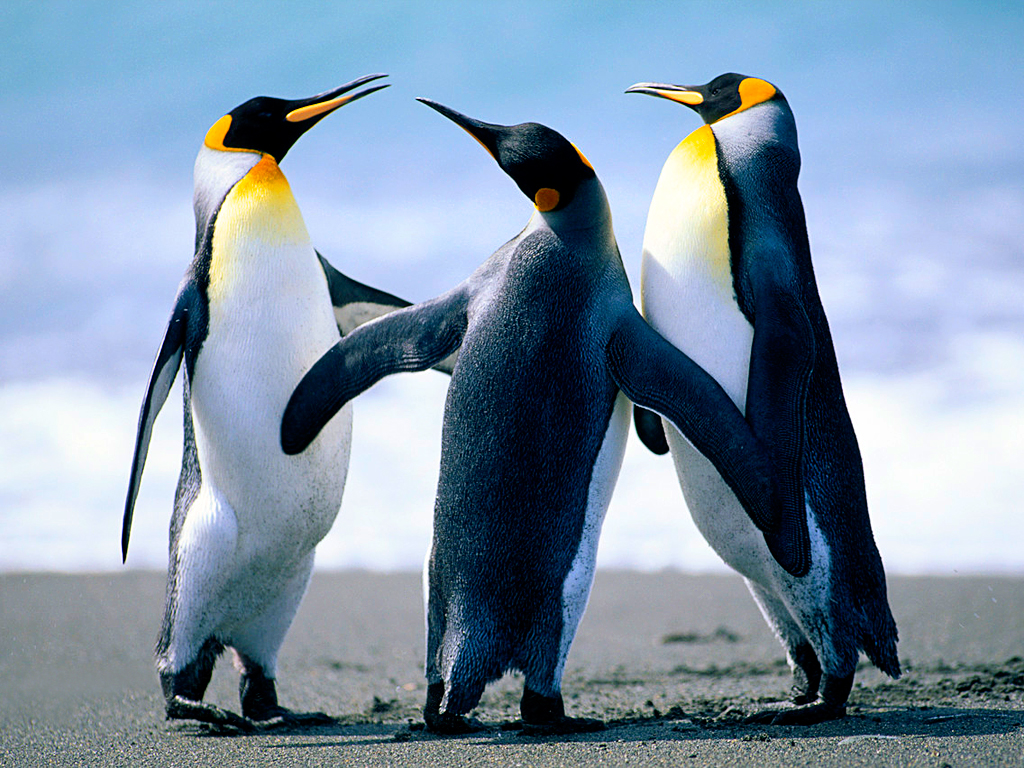
\includegraphics[scale=.50]{figures/Penguins.jpg}
\caption{TAMU figure}
\label{fig:tamu-fig6}
\end{figure}

\section{Appendix Section}


\pagebreak{}

\end{appendices}


\end{document}
